
\chapter{\label{appendix}Appendix}

\minitoc

%%%% INTRODUCTION %%%%

\begin{figure}[p]
    \centering
    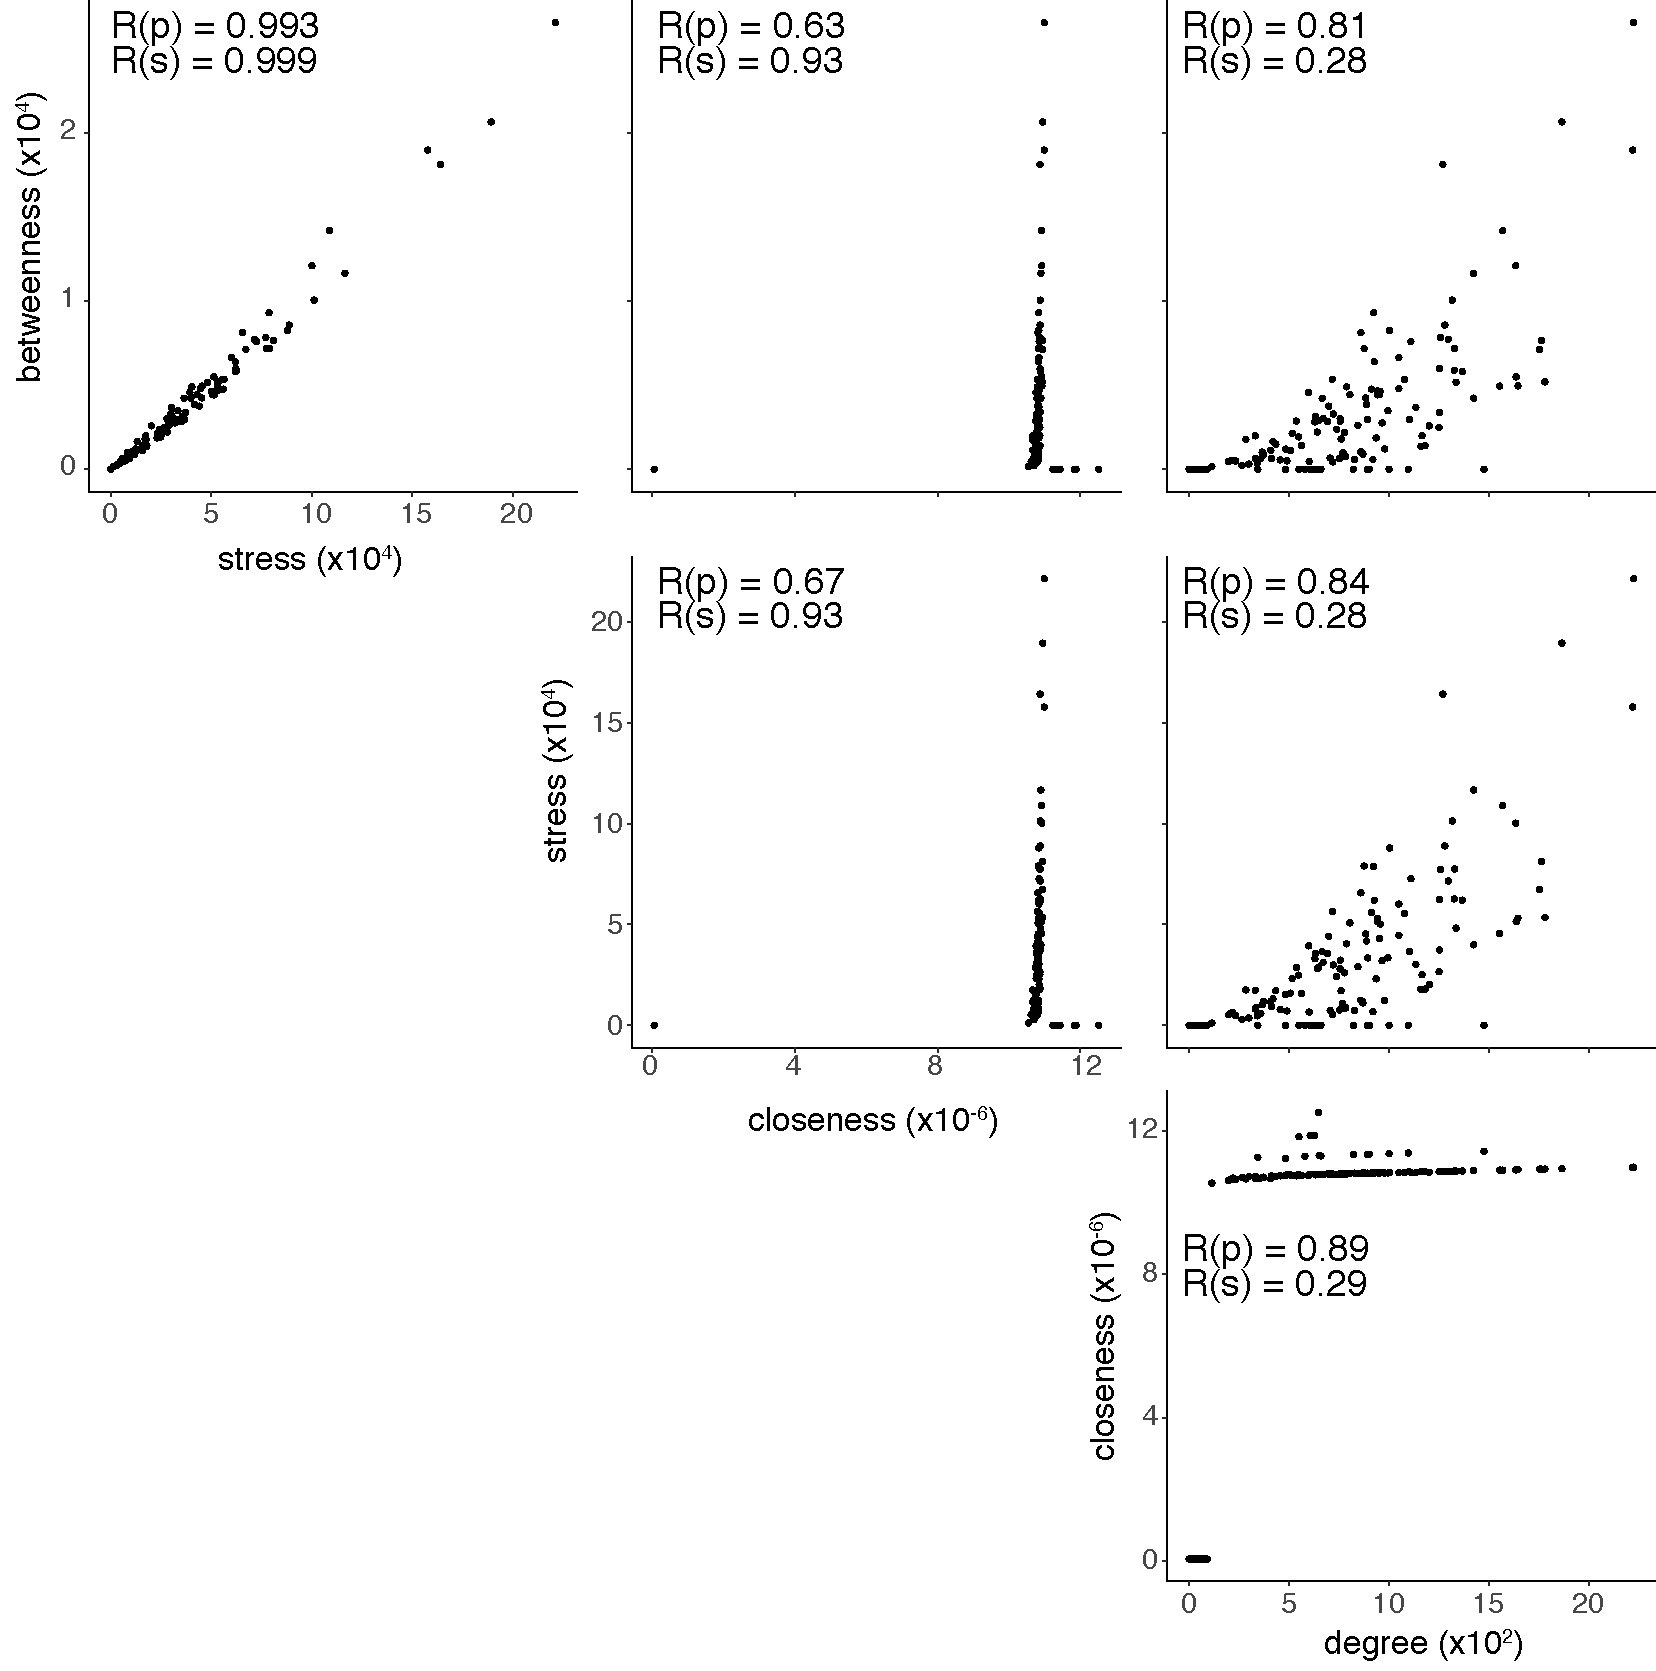
\includegraphics[width=\textwidth,height=\textheight,keepaspectratio]{figures/appendix/app_centrality-comparison.png}
    \caption[{Relationship between different centrality measures.}]
    {\textbf{Relationship between different centrality measures.} 
    Relationship between different centrality measures, as calculated using the EHT GRN.
    }
    \label{fig:app_centrality-comparison}
\end{figure}
\clearpage

%%%% METHODS %%%%

\begin{figure}[p]
    \centering
    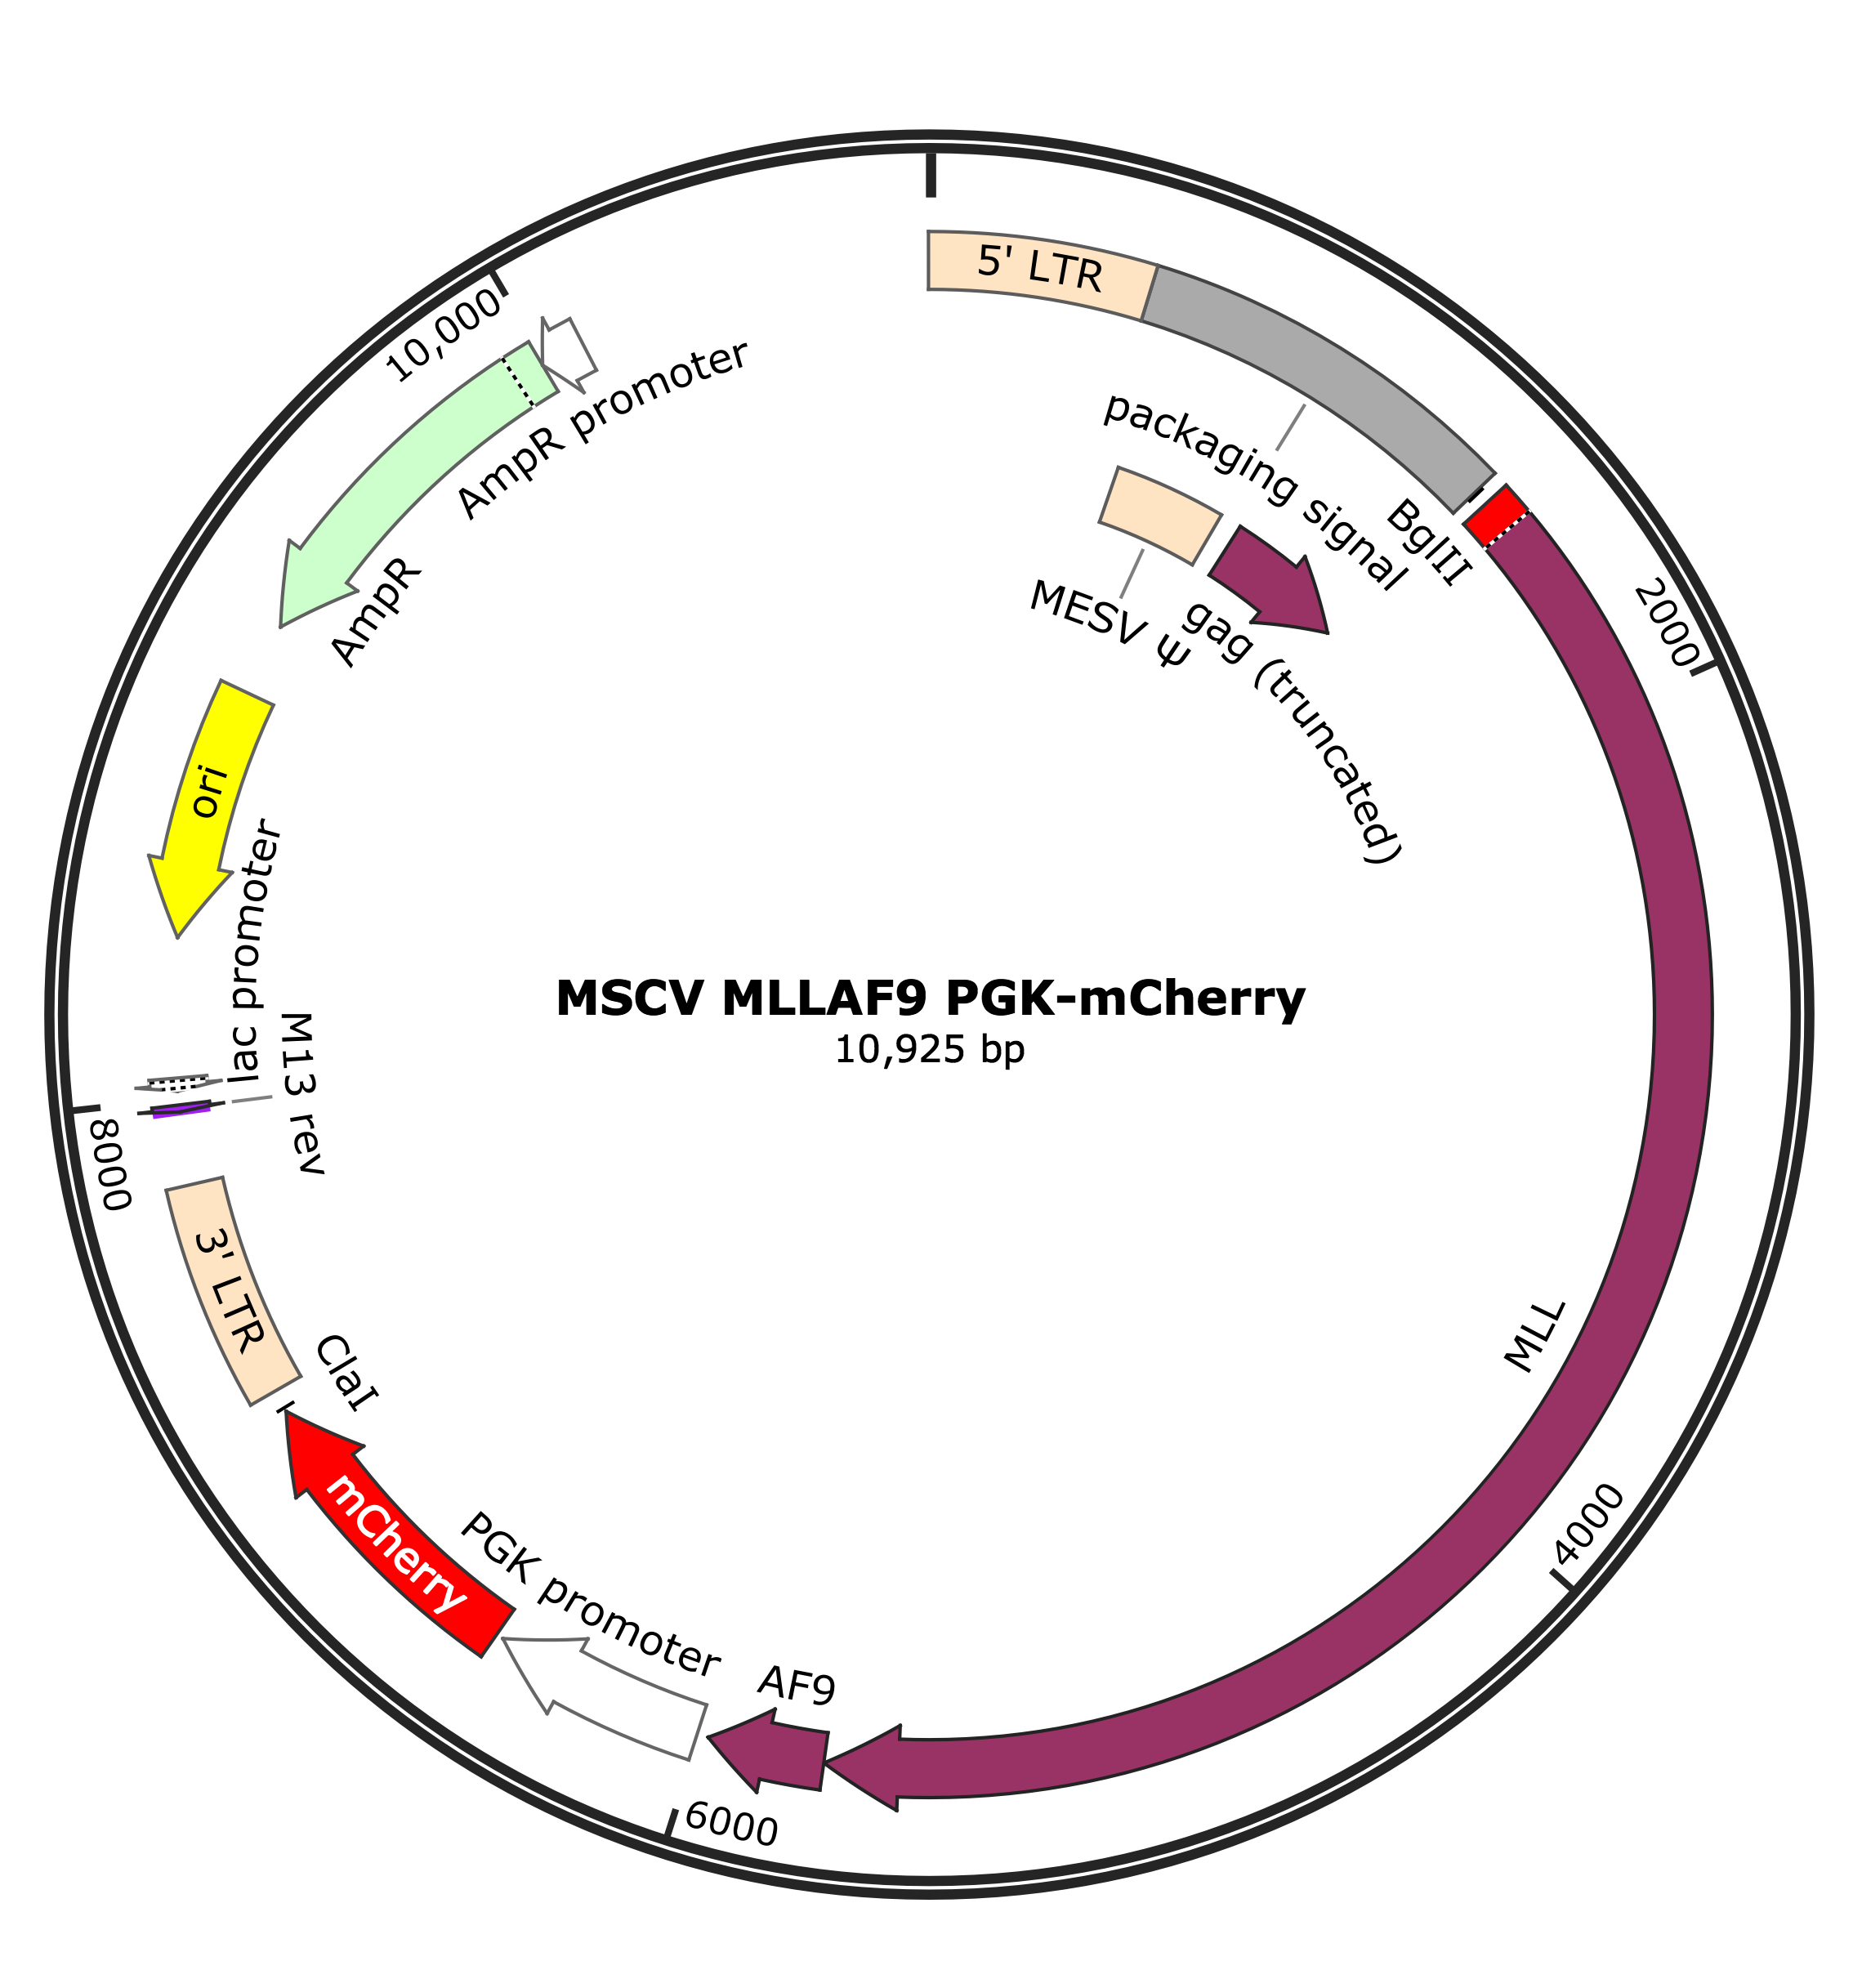
\includegraphics[width=\textwidth,height=\textheight,keepaspectratio]{figures/appendix/app_plasmid-map.png}
    \caption[{Vector map of MSCV MLL-AF9 PGK-mCherry.}]
    {\textbf{Vector map of MSCV MLL-AF9 PGK-mCherry.} 
    \textit{Vector and vector map generated by I-Jun Lau.}
    }
    \label{fig:app_plasmid-map}
\end{figure}
\clearpage

\begin{figure}[p]
    \centering
    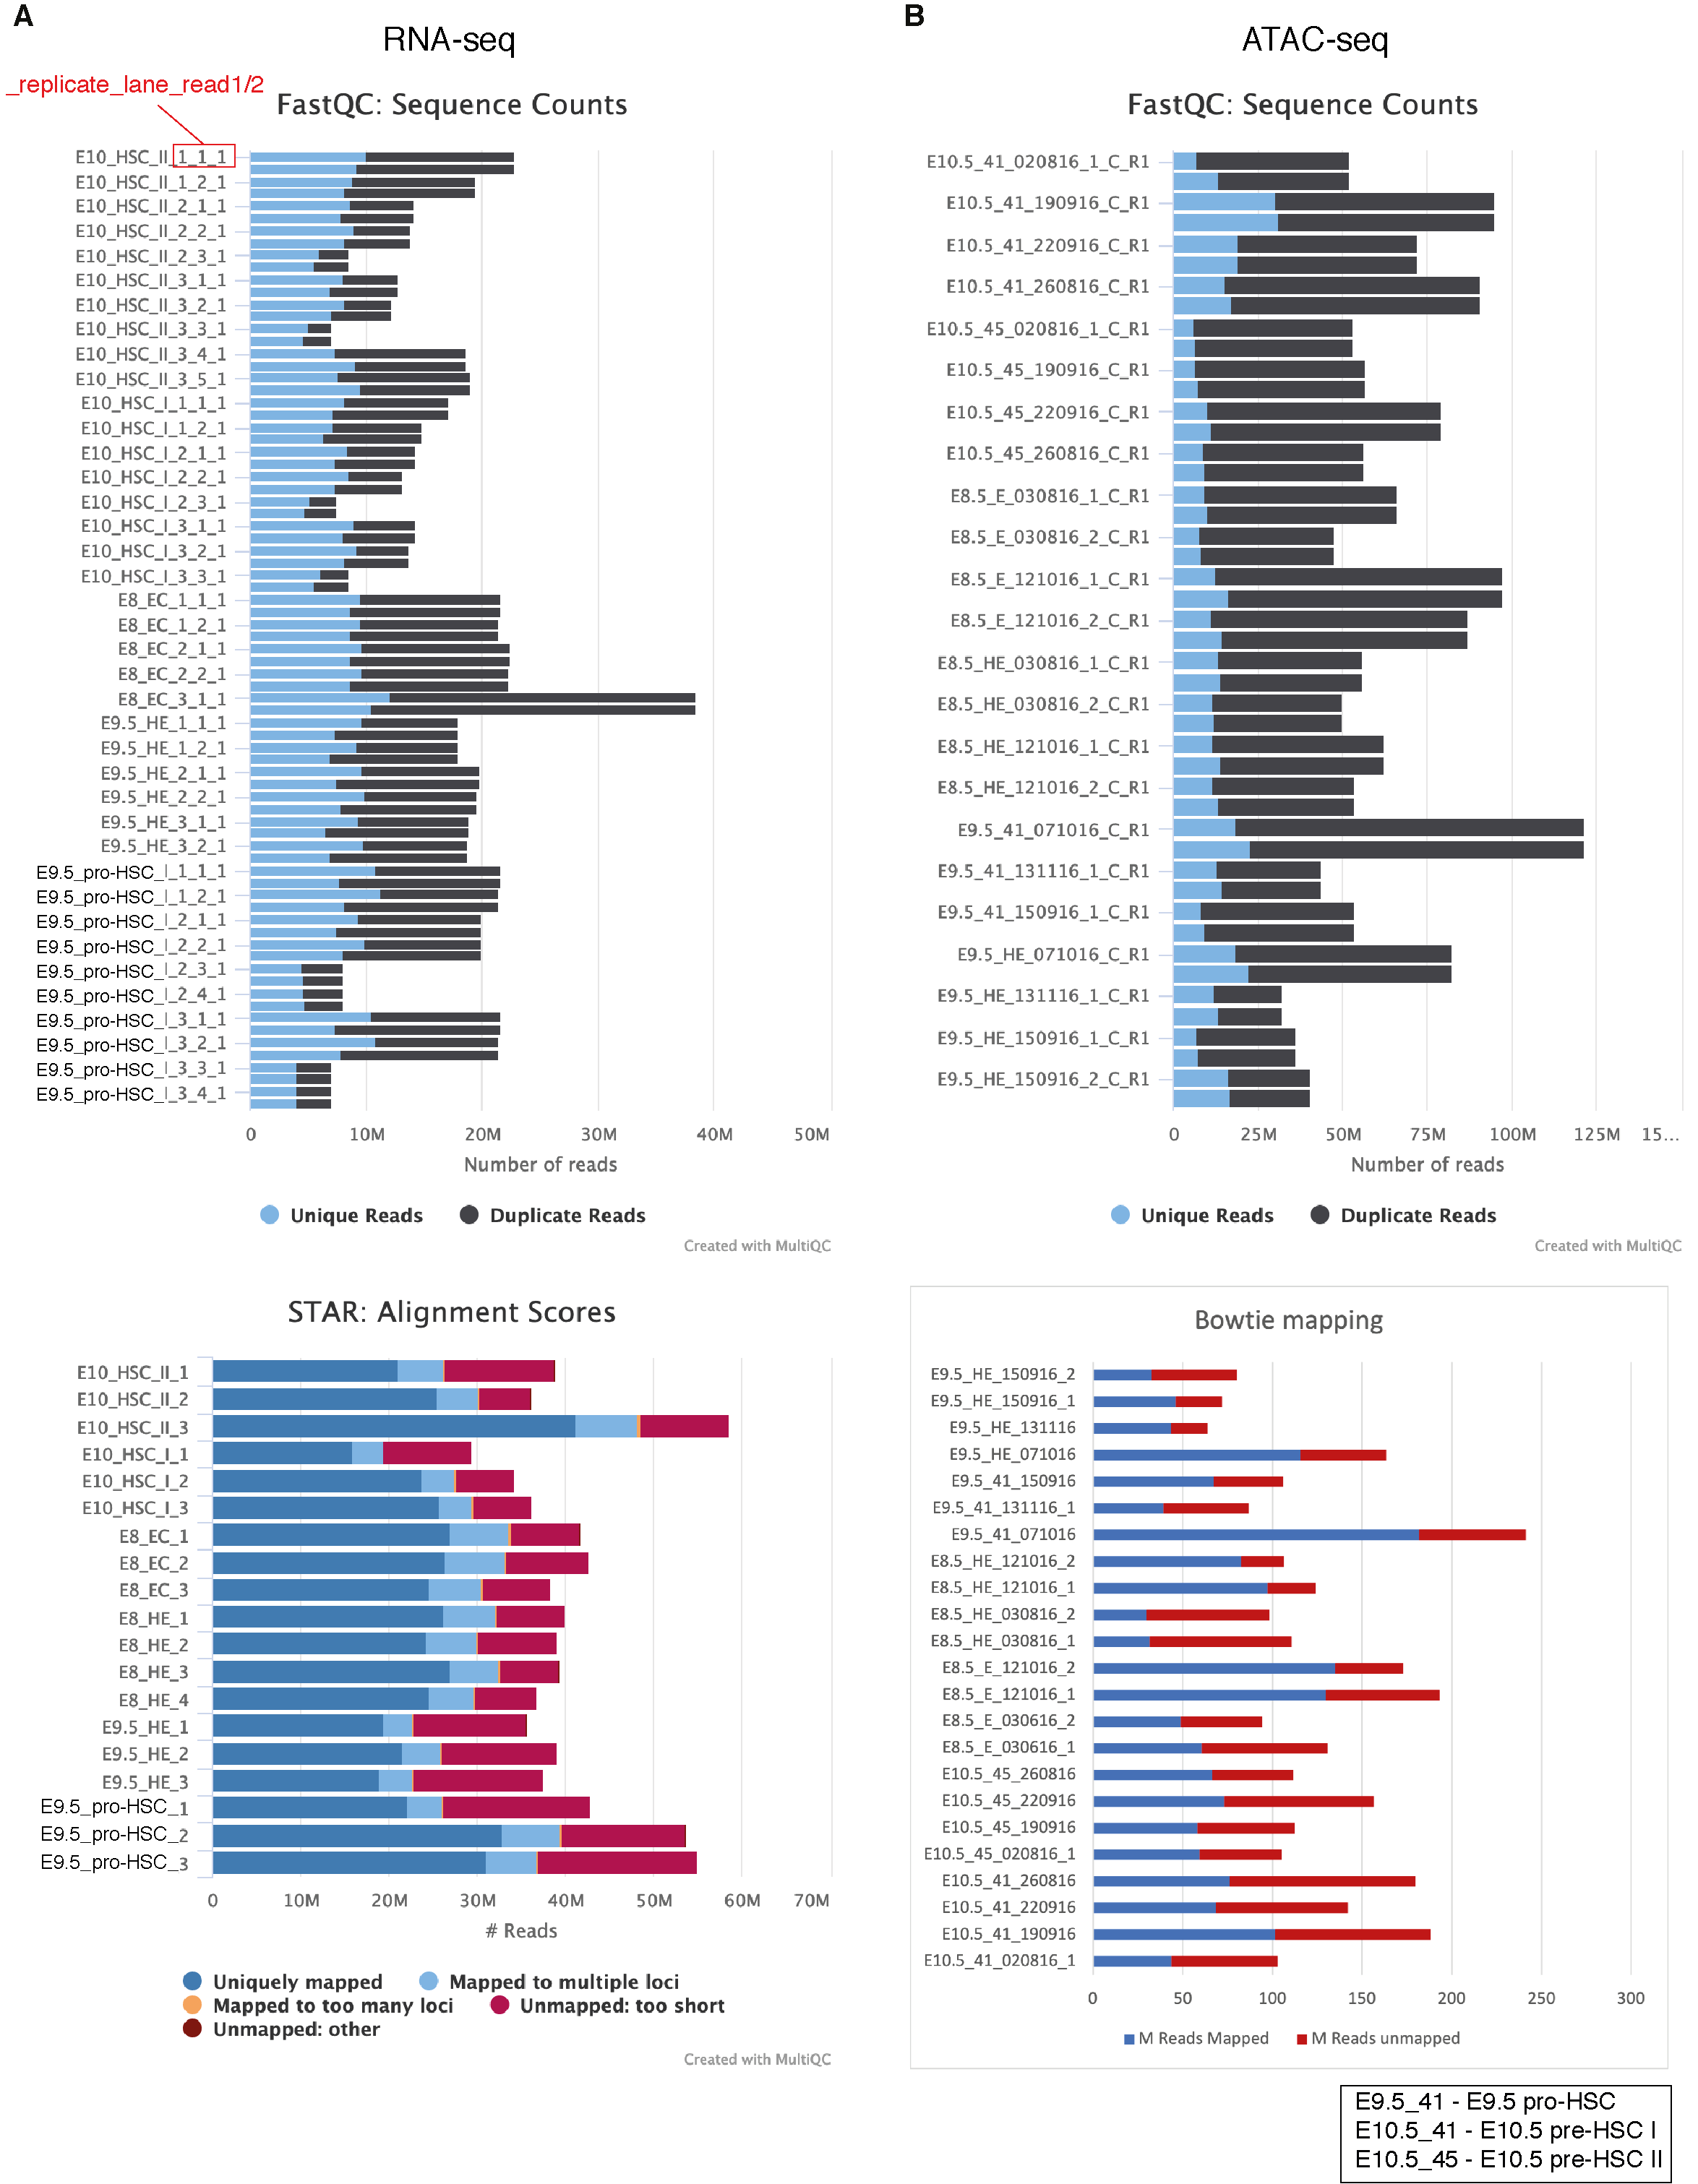
\includegraphics[width=0.9\textwidth,height=0.9\textheight,keepaspectratio]{figures/appendix/app_eht-qc.png}
    \caption[{Quality control plots for EHT RNA-seq and ATAC-seq.}]
    {\textbf{Quality control plots for EHT RNA-seq and ATAC-seq.} 
    \textbf{(A-B)} FastQC breakdown of read duplication, STAR mapping metrics, and Bowtie2 mapping metrics for RNA-seq (A) and ATAC-seq (B).
    }
    \label{fig:app_eht-qc}
\end{figure}
\clearpage

\begin{figure}[p]
    \centering
    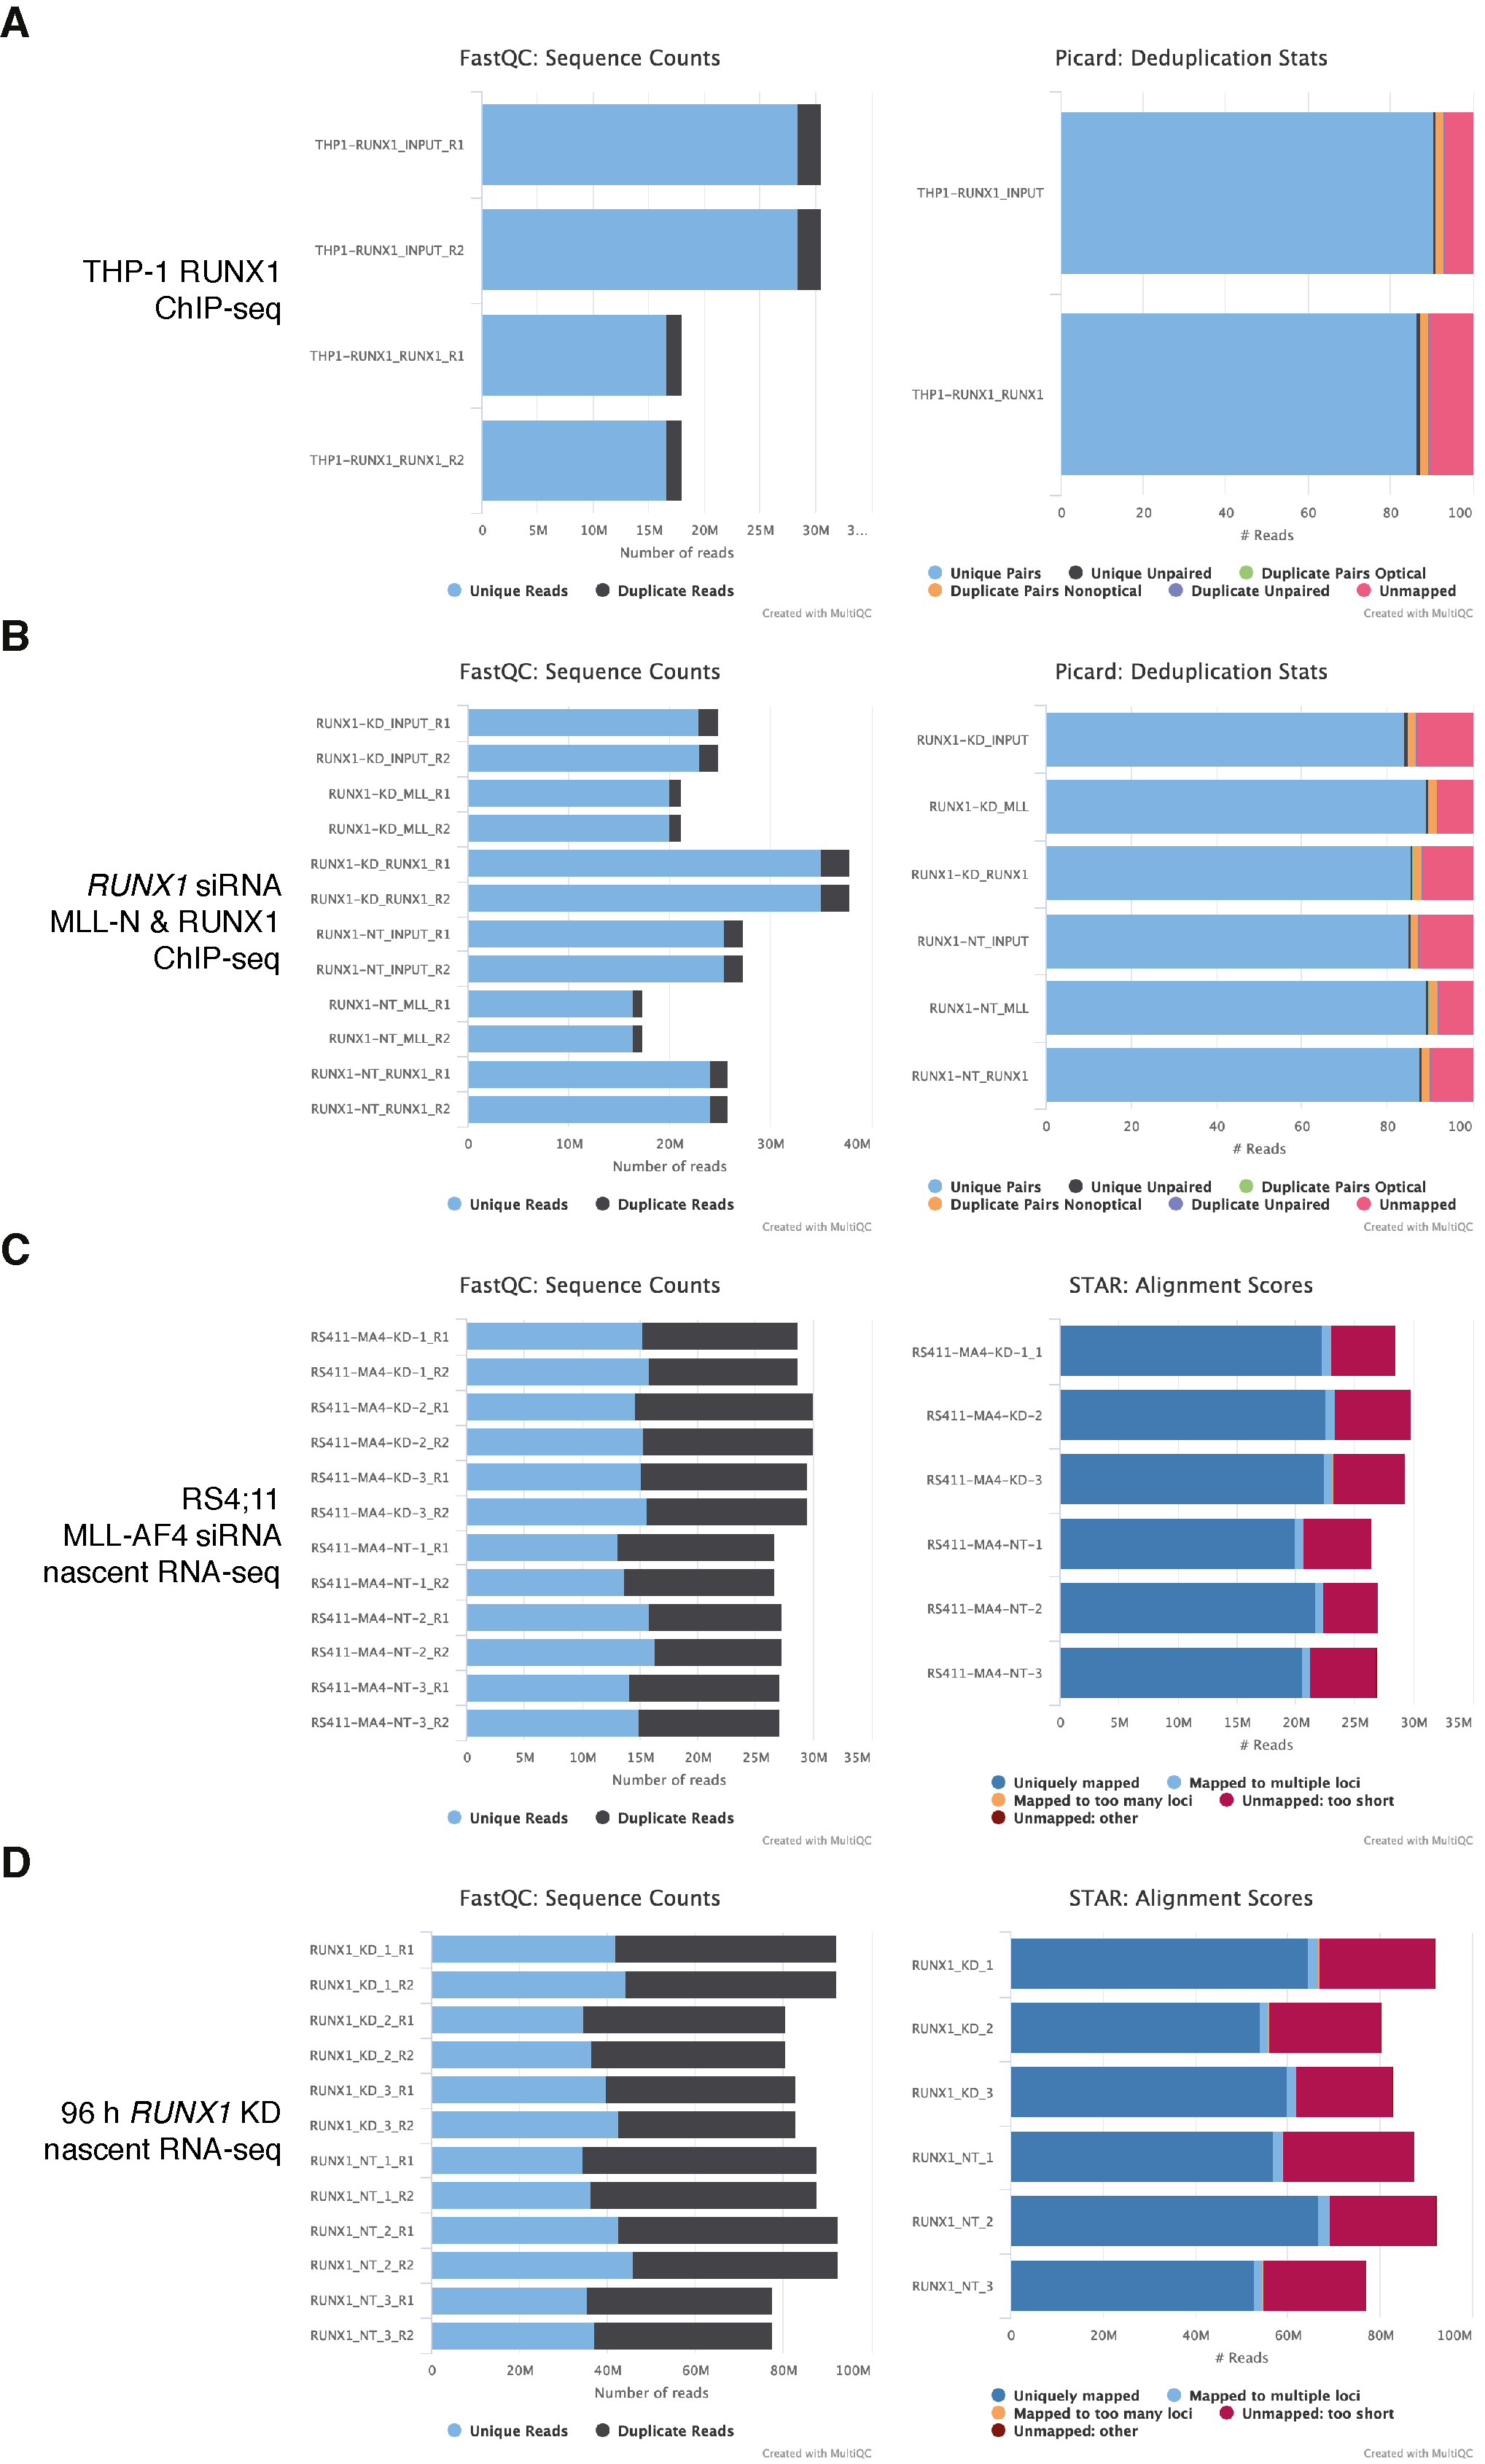
\includegraphics[width=0.9\textwidth,height=0.9\textheight,keepaspectratio]{figures/appendix/app_chapter4-qc.png}
    \caption[{FastQC and mapping statistics for unpublished datasets in chapter 4.}]
    {\textbf{FastQC and mapping statistics for unpublished datasets in chapter 4.} 
    \textit{Legend continued on next page.}
    }
    \label{fig:app_chapter4-qc}
\end{figure}
\clearpage

\begin{figure}[!b]
    \ContinuedFloat
    \hrule
    \vspace{5mm}
    \caption[]
    {\textit{Legend continued from previous page}. 
    FastQC (left) and read mapping statistics (right) for THP-1 RUNX1 ChIP-seq (A), SEM 96 h \textit{RUNX1} KD MLL-N and RUNX1 ChIP-seq (B), RS4;11 96 h \textit{MLL-AF4} KD nascent RNA-seq (C), and SEM 96 h \textit{RUNX1} KD nascent RNA-seq (D). \textit{Nascent RNA-seq data in (D) was generated by M. Tapia (Milne lab), and analysed by me}. 
    }
\end{figure}
%\vspace*{9in}
\clearpage

\begin{figure}[p]
    \centering
    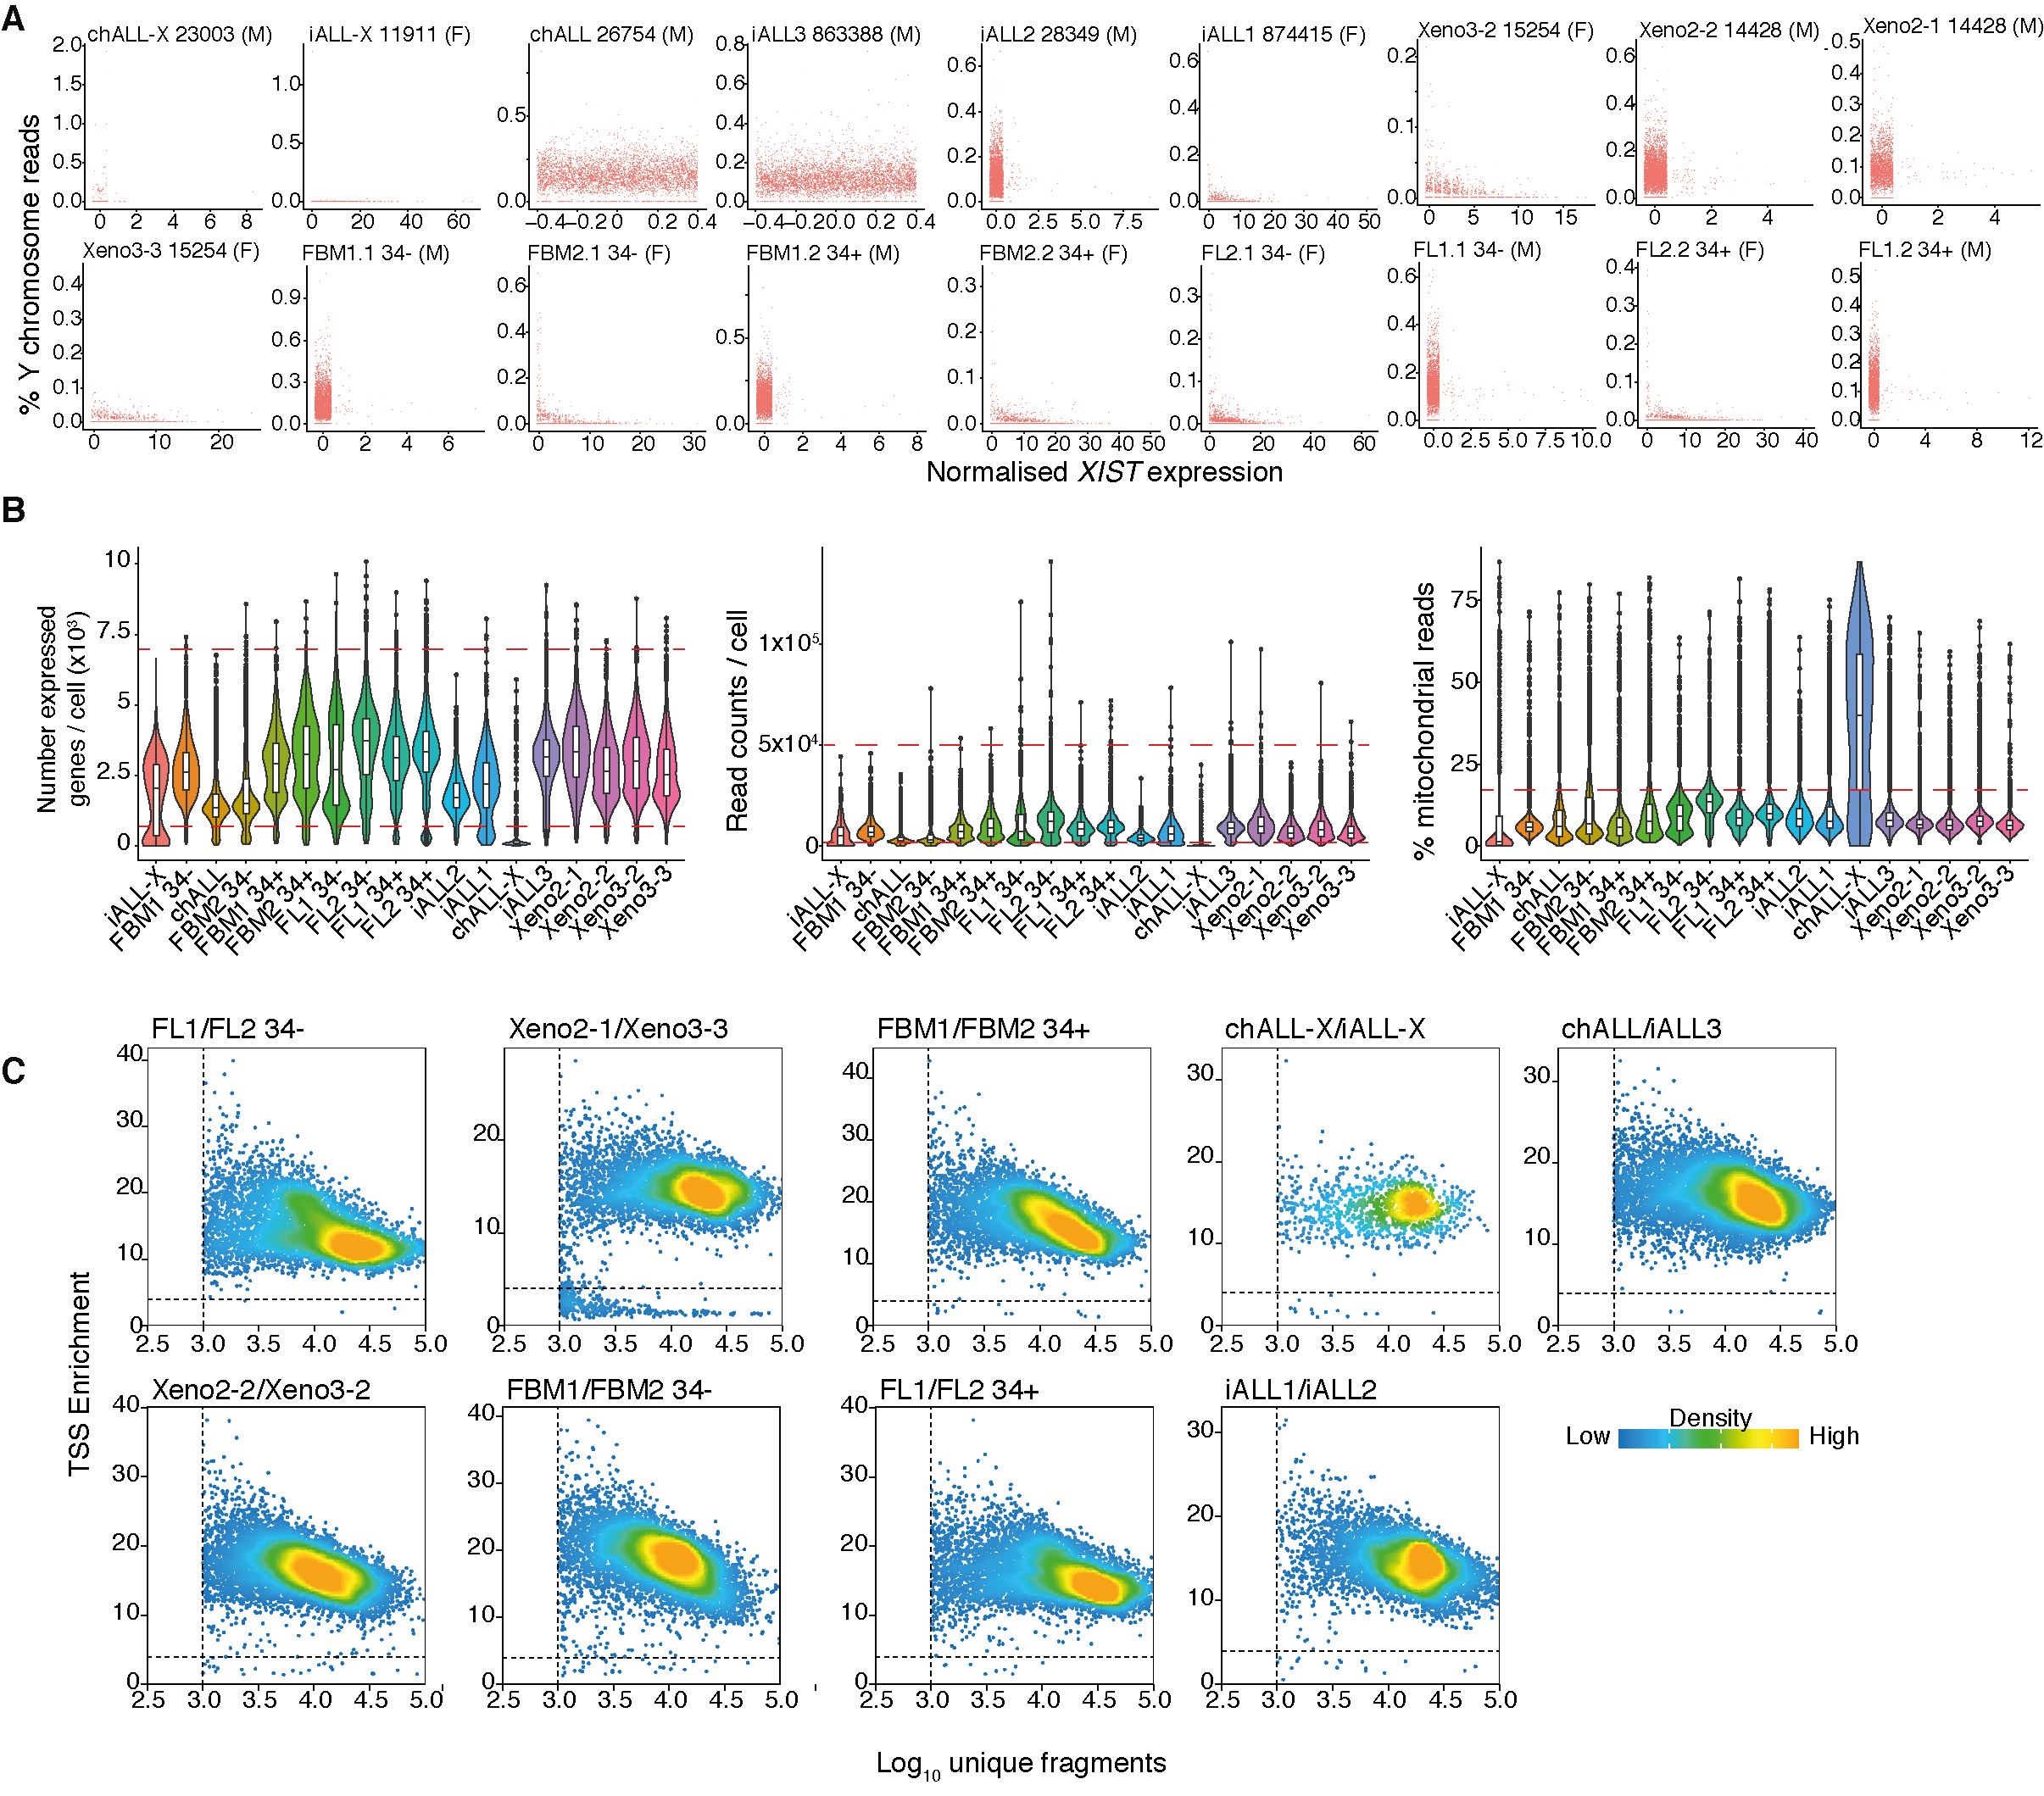
\includegraphics[width=\textwidth,height=\textheight,keepaspectratio]{figures/appendix/app_multiome-qc.png}
    \caption[{RNA+ATAC multiome quality control plots.}]
    {\textbf{RNA+ATAC multiome quality control plots.} 
    \textbf{(A)} Single cell Feature plots showing \textit{XIST} expression against percentage of reads in Y chromosome. Data used to judge gender of the population, for deconvoluting multiplexed samples.
    \textbf{(B)} Violin and boxplots showing distribution of total detected genes, total read count, and percentage mitochondrial reads. Red dashed lines indicate quality thresholds (see methods).
    \textbf{(C)} ArchR quality control plots, showing total unique fragments against TSS enrichment. Dashed line indicates quality thresholds (see methods). 
    \textit{Plots and data filtering in C performed by Alastair Smith.}
    }
    \label{fig:app_multiome-qc}
\end{figure}
\clearpage

\begin{figure}[p]
    \centering
    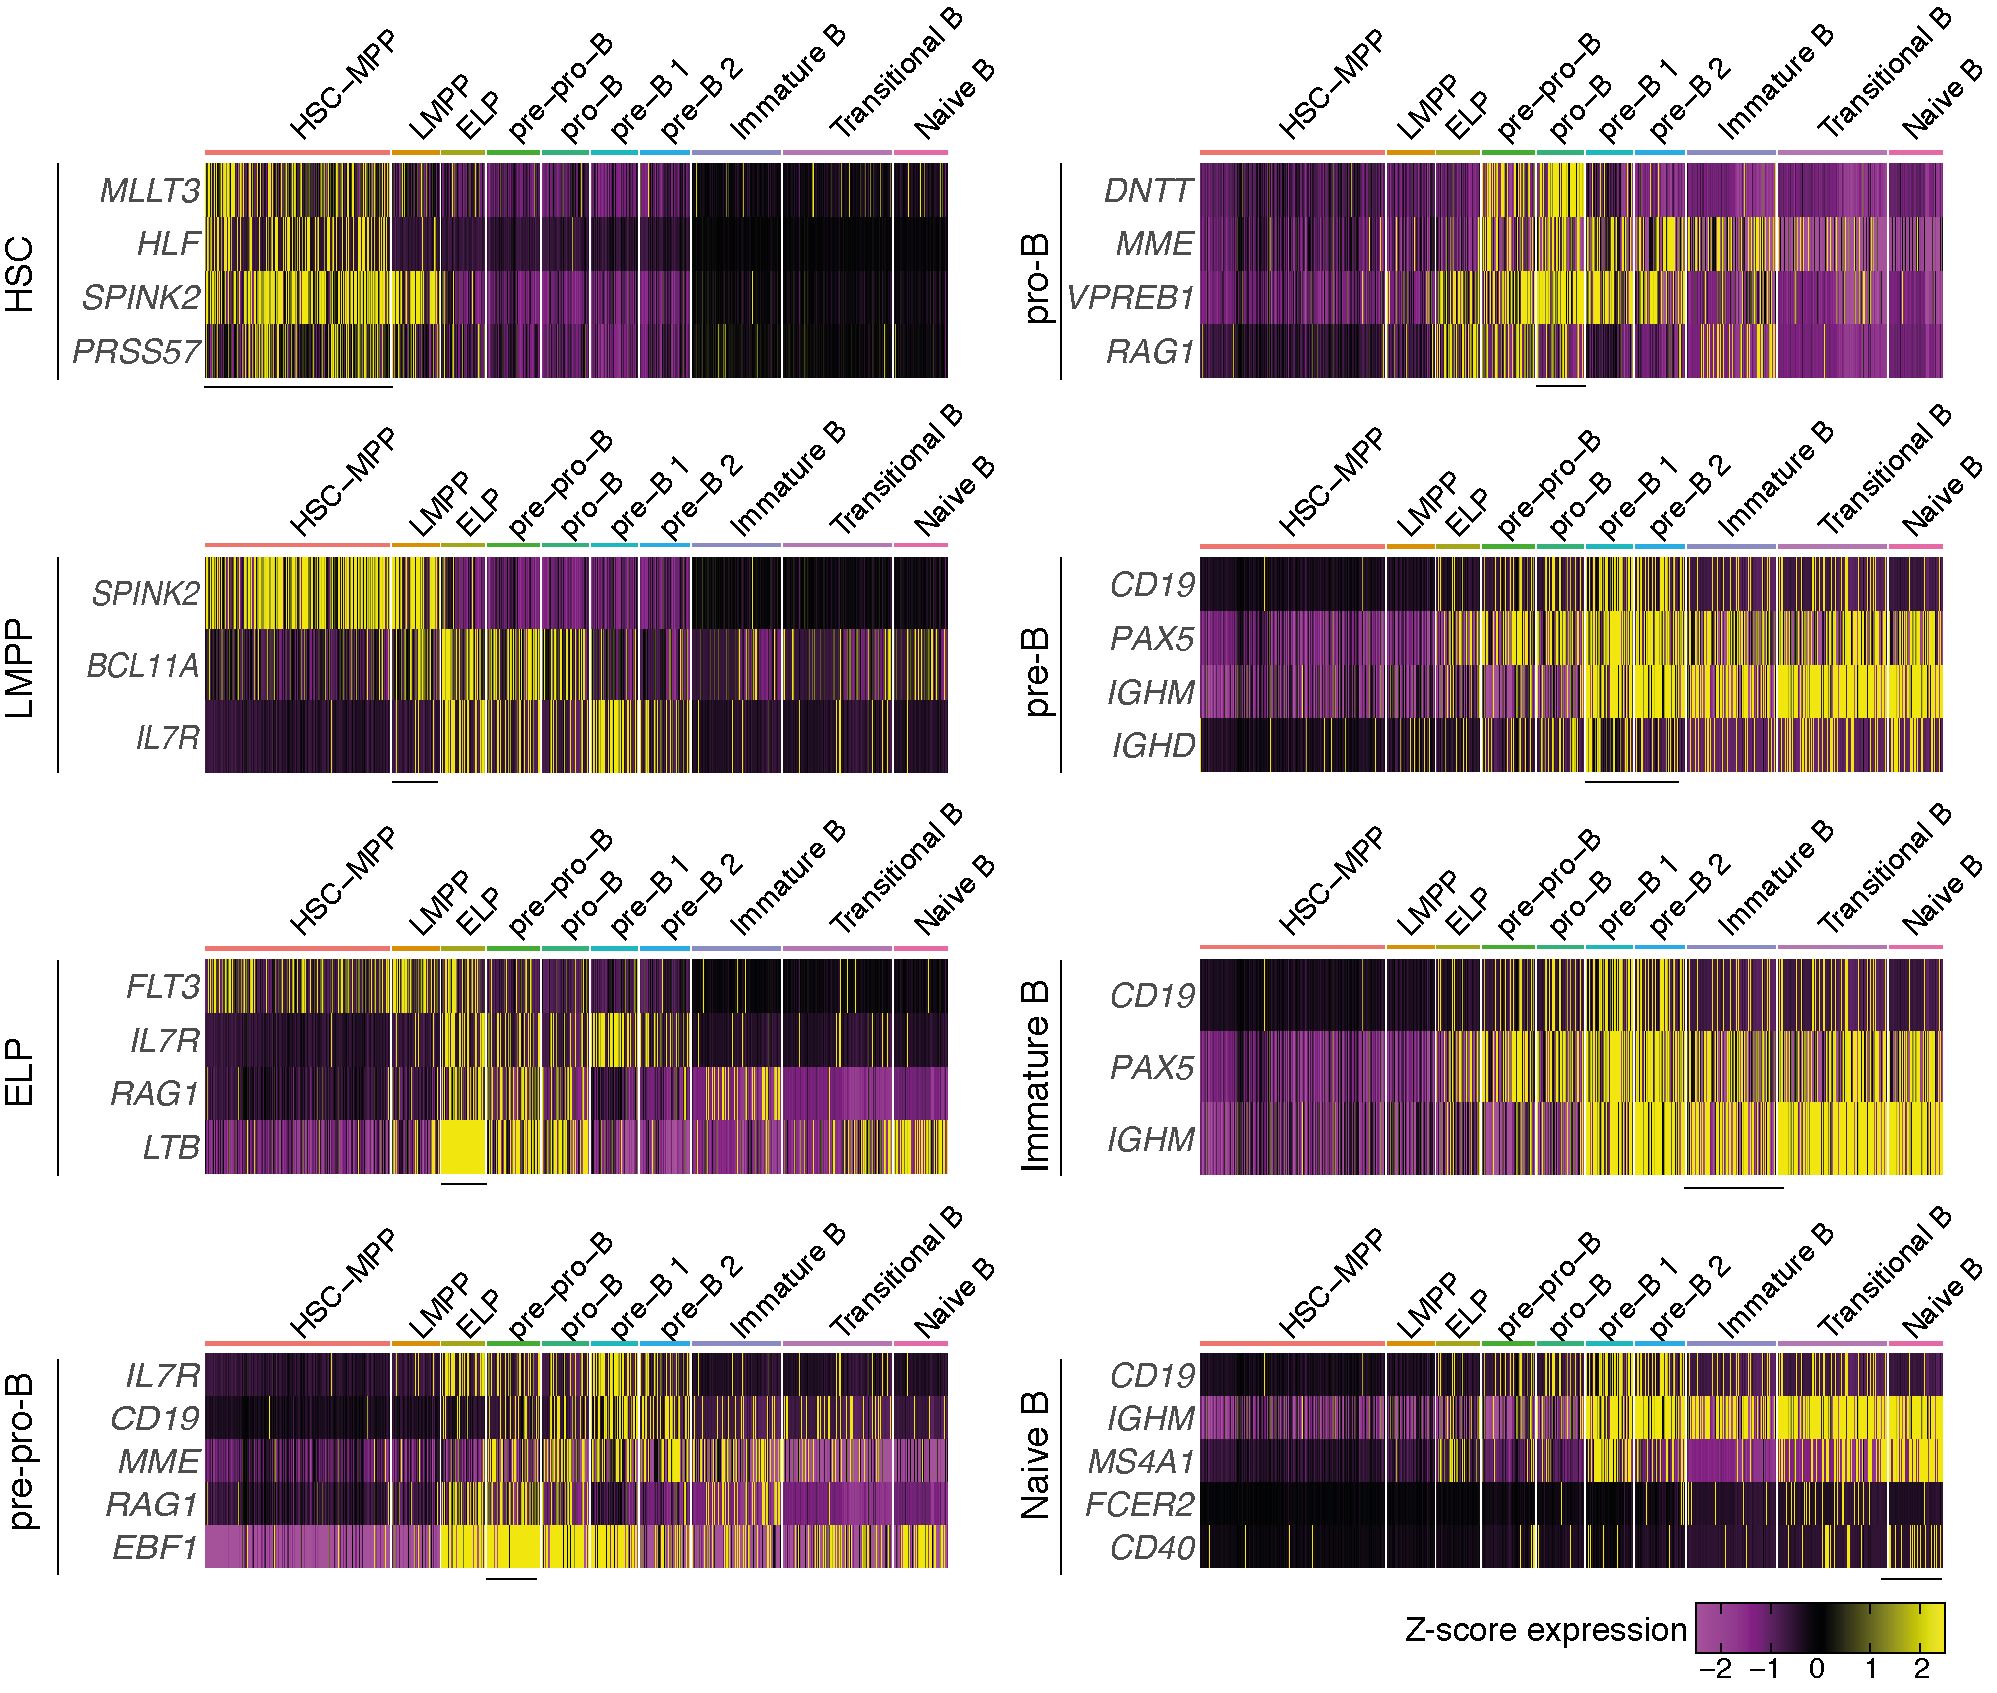
\includegraphics[width=\textwidth,height=\textheight,keepaspectratio]{figures/appendix/app_multiome-lineage-markers.png}
    \caption[{Sc-multiome lineage markers defining B progenitor populations.}]
    {\textbf{Sc-multiome lineage markers defining B progenitor populations.} 
    Heatmap of z-score scaled normalised gene expression over labelled B progenitor populations. Genes shown are transcriptional markers differentiating B progenitor populations \citep{jardine_blood_2021, suo_mapping_2022}. Note transitional B population is defined as such as it is a cluster between immature and Naive B populations.
    }
    \label{fig:app_multiome-lineage-markers}
\end{figure}
\clearpage

\begin{figure}[p]
    \centering
    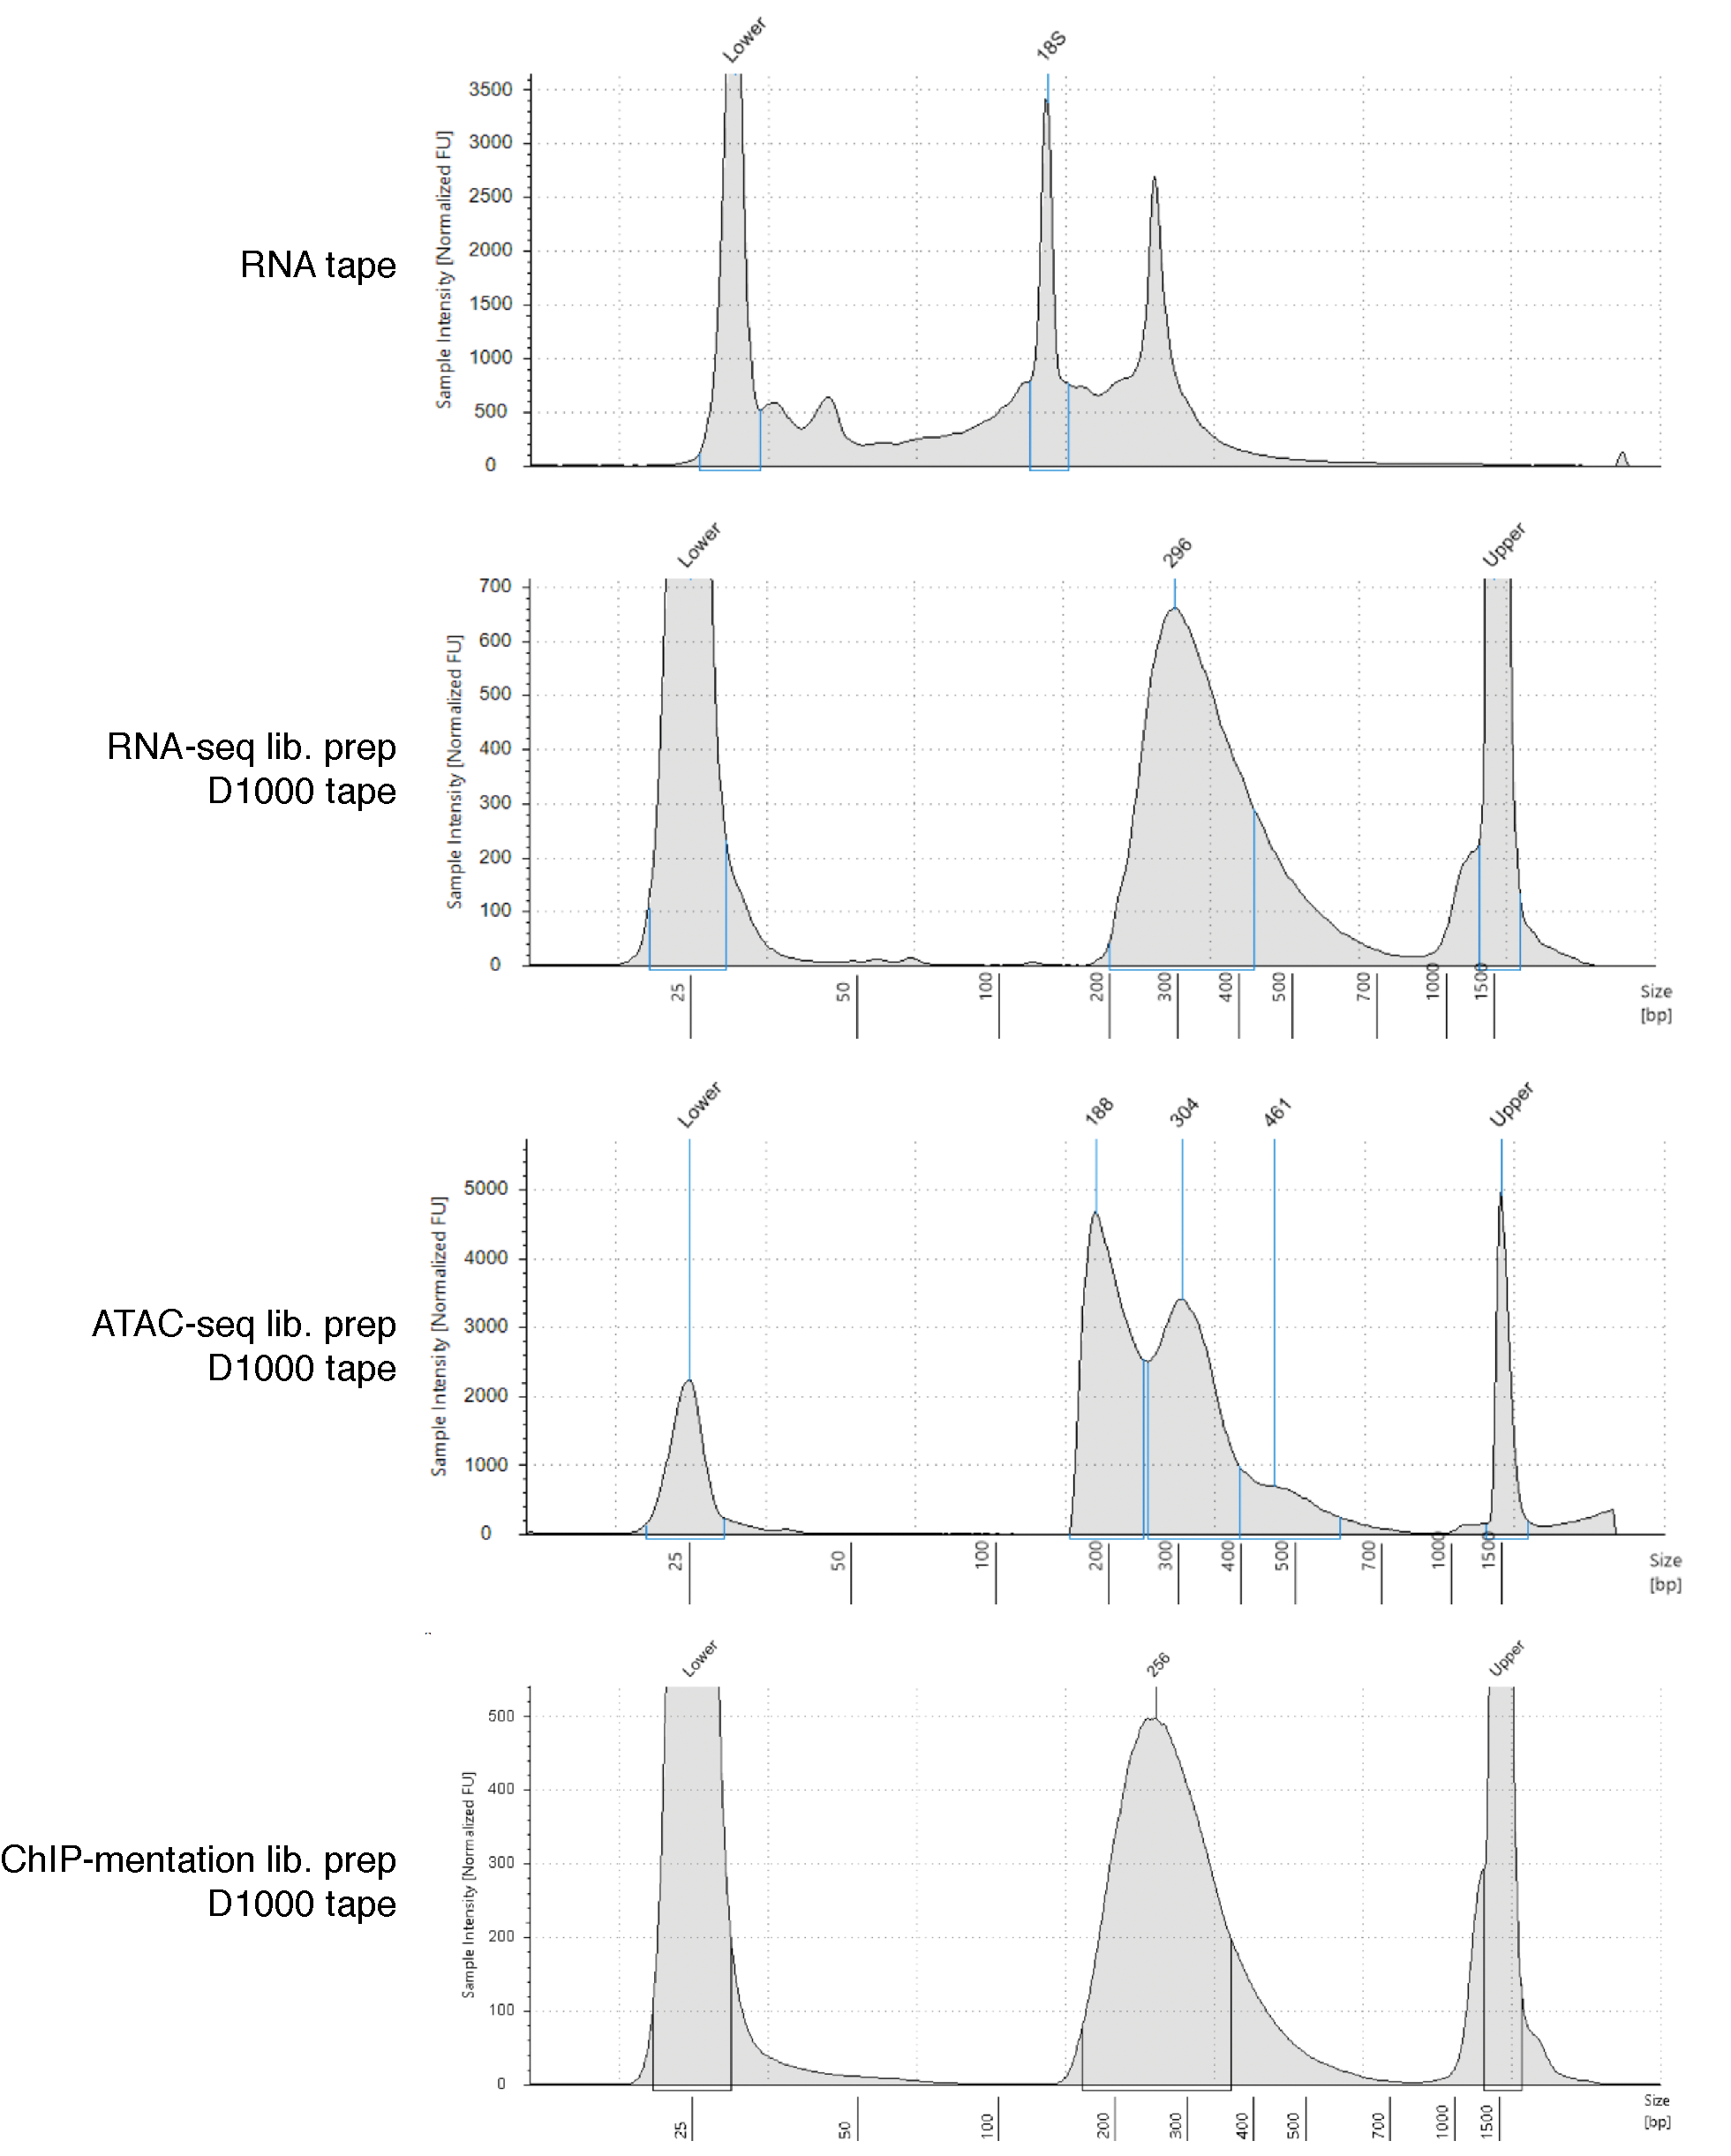
\includegraphics[width=\textwidth,height=\textheight,keepaspectratio]{figures/appendix/app_methocult-tapestation.png}
    \caption[{Tapestation traces for MLL-AF9 GMP MethoCult replating.}]
    {\textbf{Tapestation traces for MLL-AF9 GMP MethoCult replating.} 
    Representative tapestation traces for RNA (top), and RNA-seq, ATAC-seq and ChIP-mentation libraries (bottom), generated from the MLL-AF9 GMP MethoCult replating experiment.
    }
    \label{fig:app_methocult-tapestation}
\end{figure}
\clearpage

\begin{figure}[p]
    \centering
    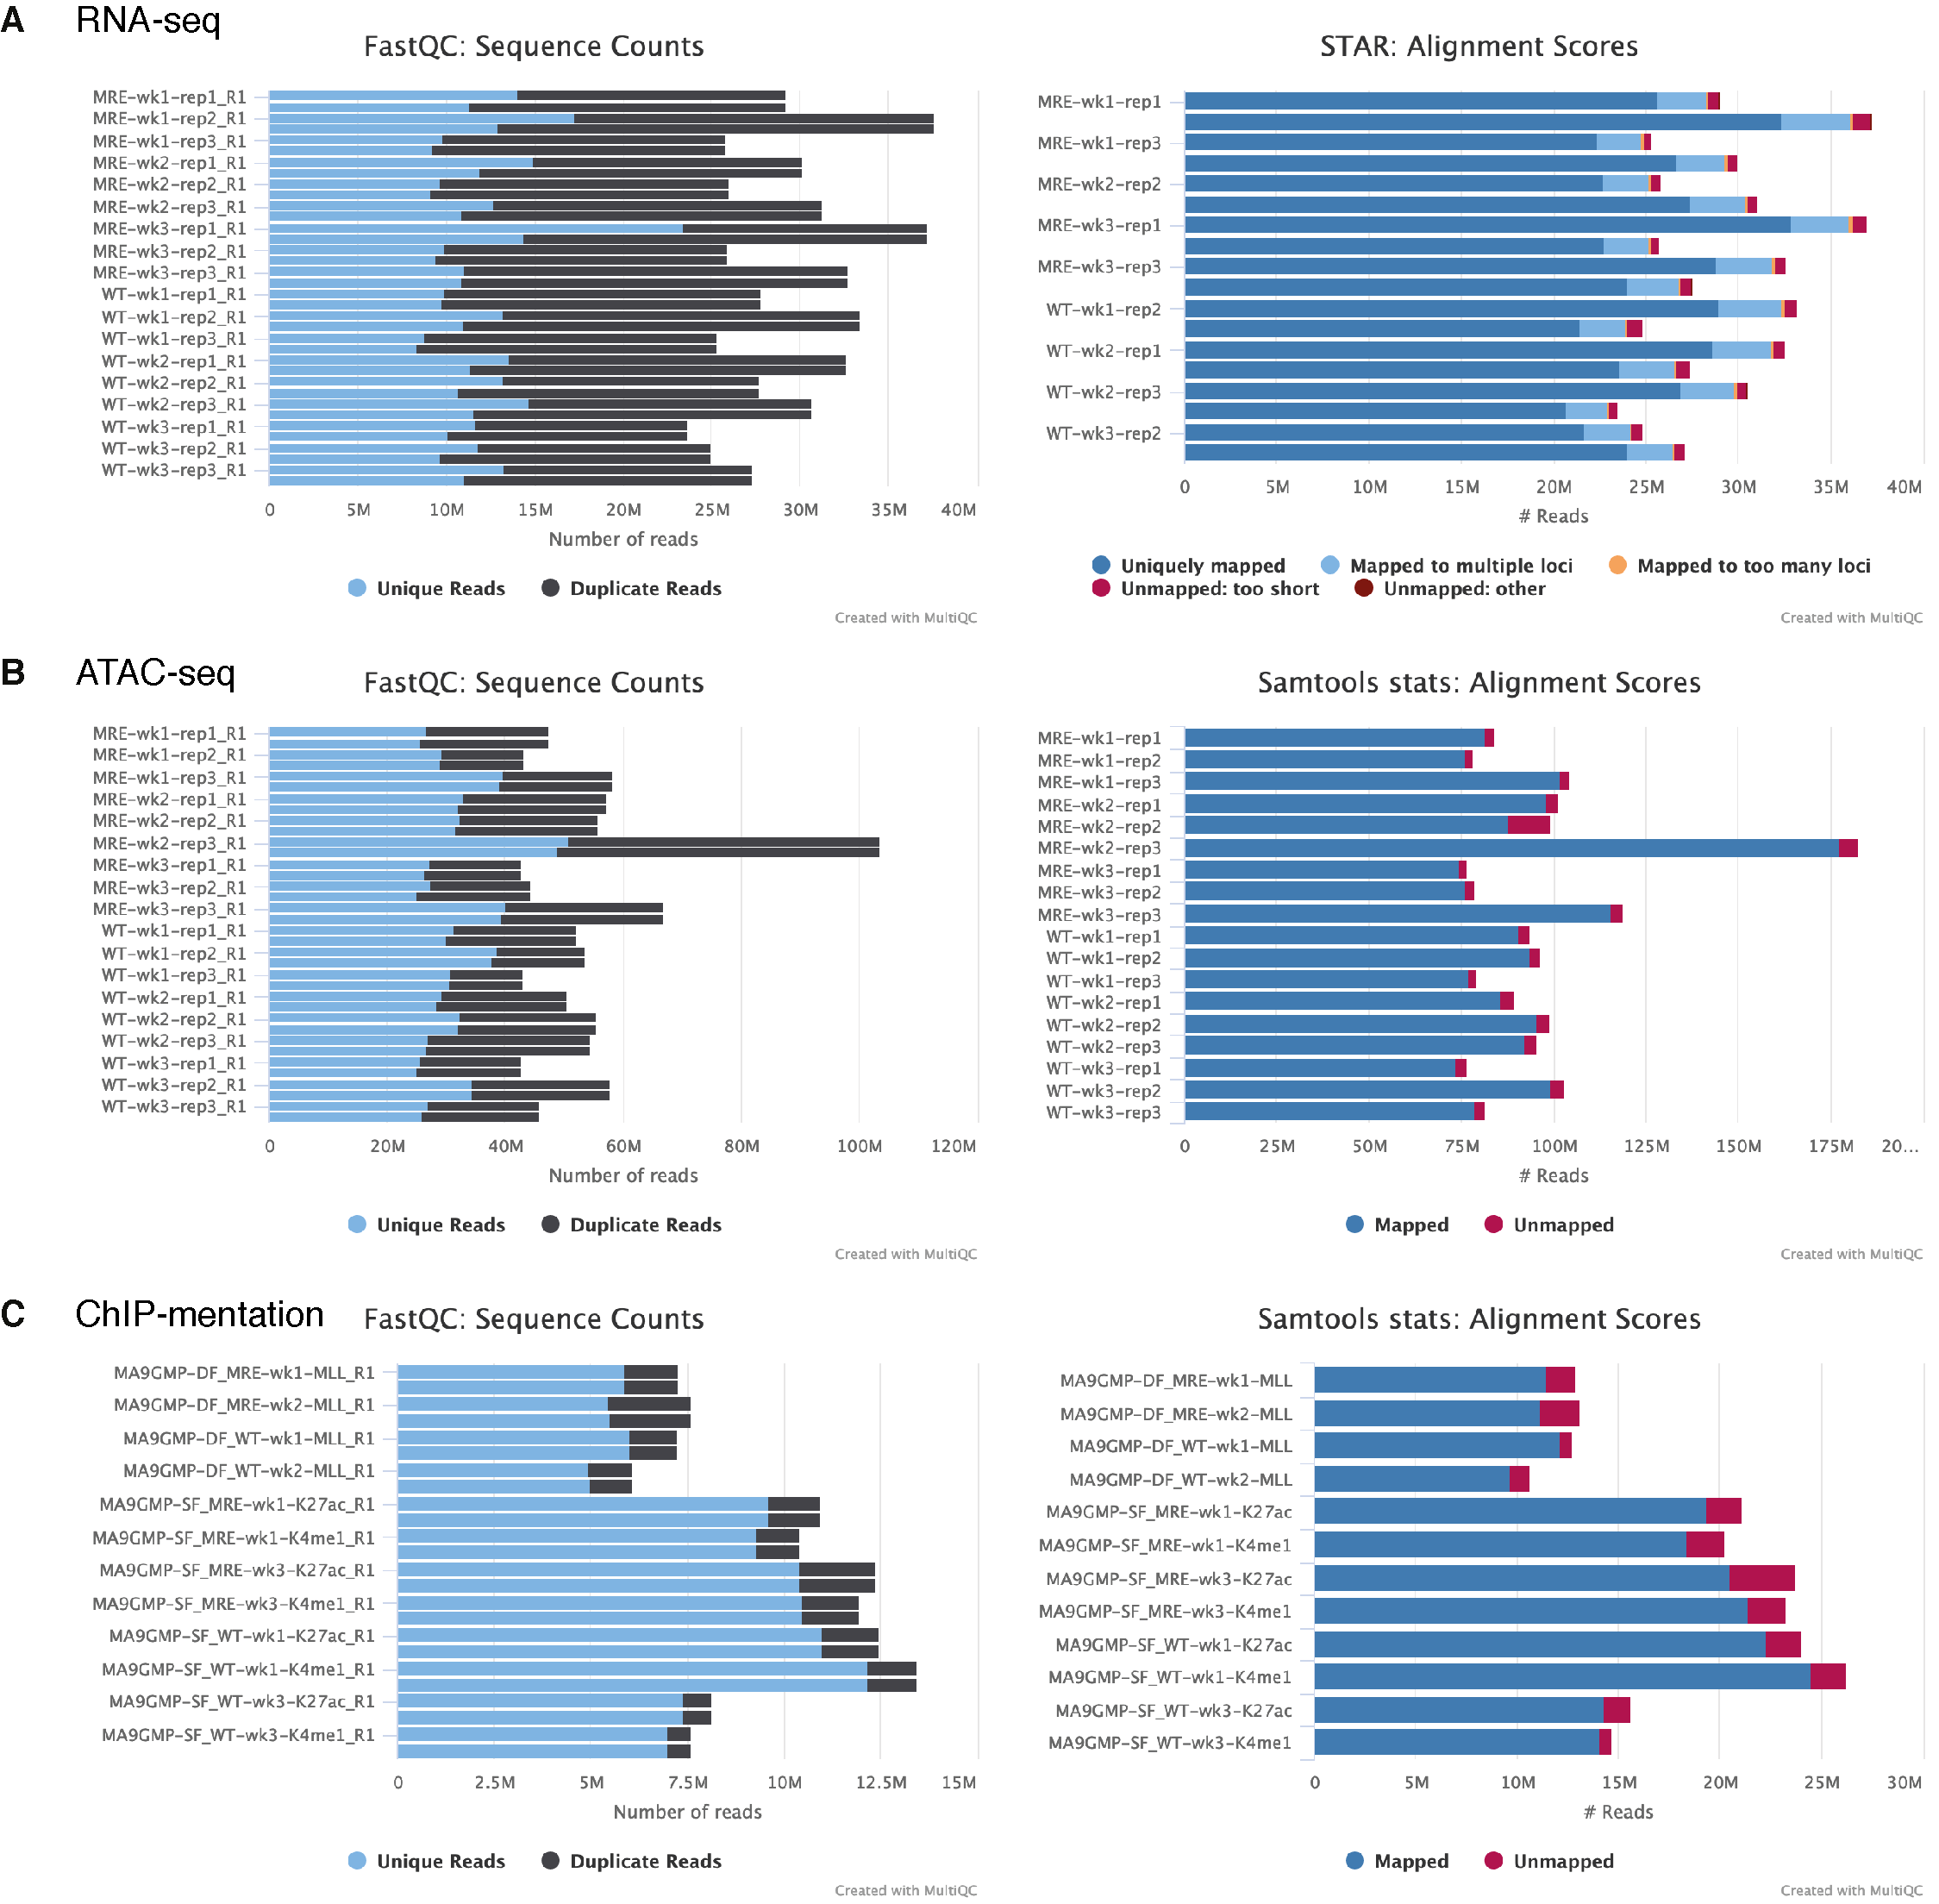
\includegraphics[width=\textwidth,height=\textheight,keepaspectratio]{figures/appendix/app_methocult-QC.png}
    \caption[{FastQC and mapping statistics for MLL-AF9 GMP MethoCult replating.}]
    {\textbf{FastQC and mapping statistics for MLL-AF9 GMP MethoCult replating.} 
    FastQC (left) and read mapping statistics (right) for RNA-seq (A), ATAC-seq (B) and ChIP-mentation (C) data, generated from the MLL-AF9 GMP MethoCult replating experiment. 
    }
    \label{fig:app_methocult-qc}
\end{figure}
\clearpage




















\begin{figure}[p]
    \centering
    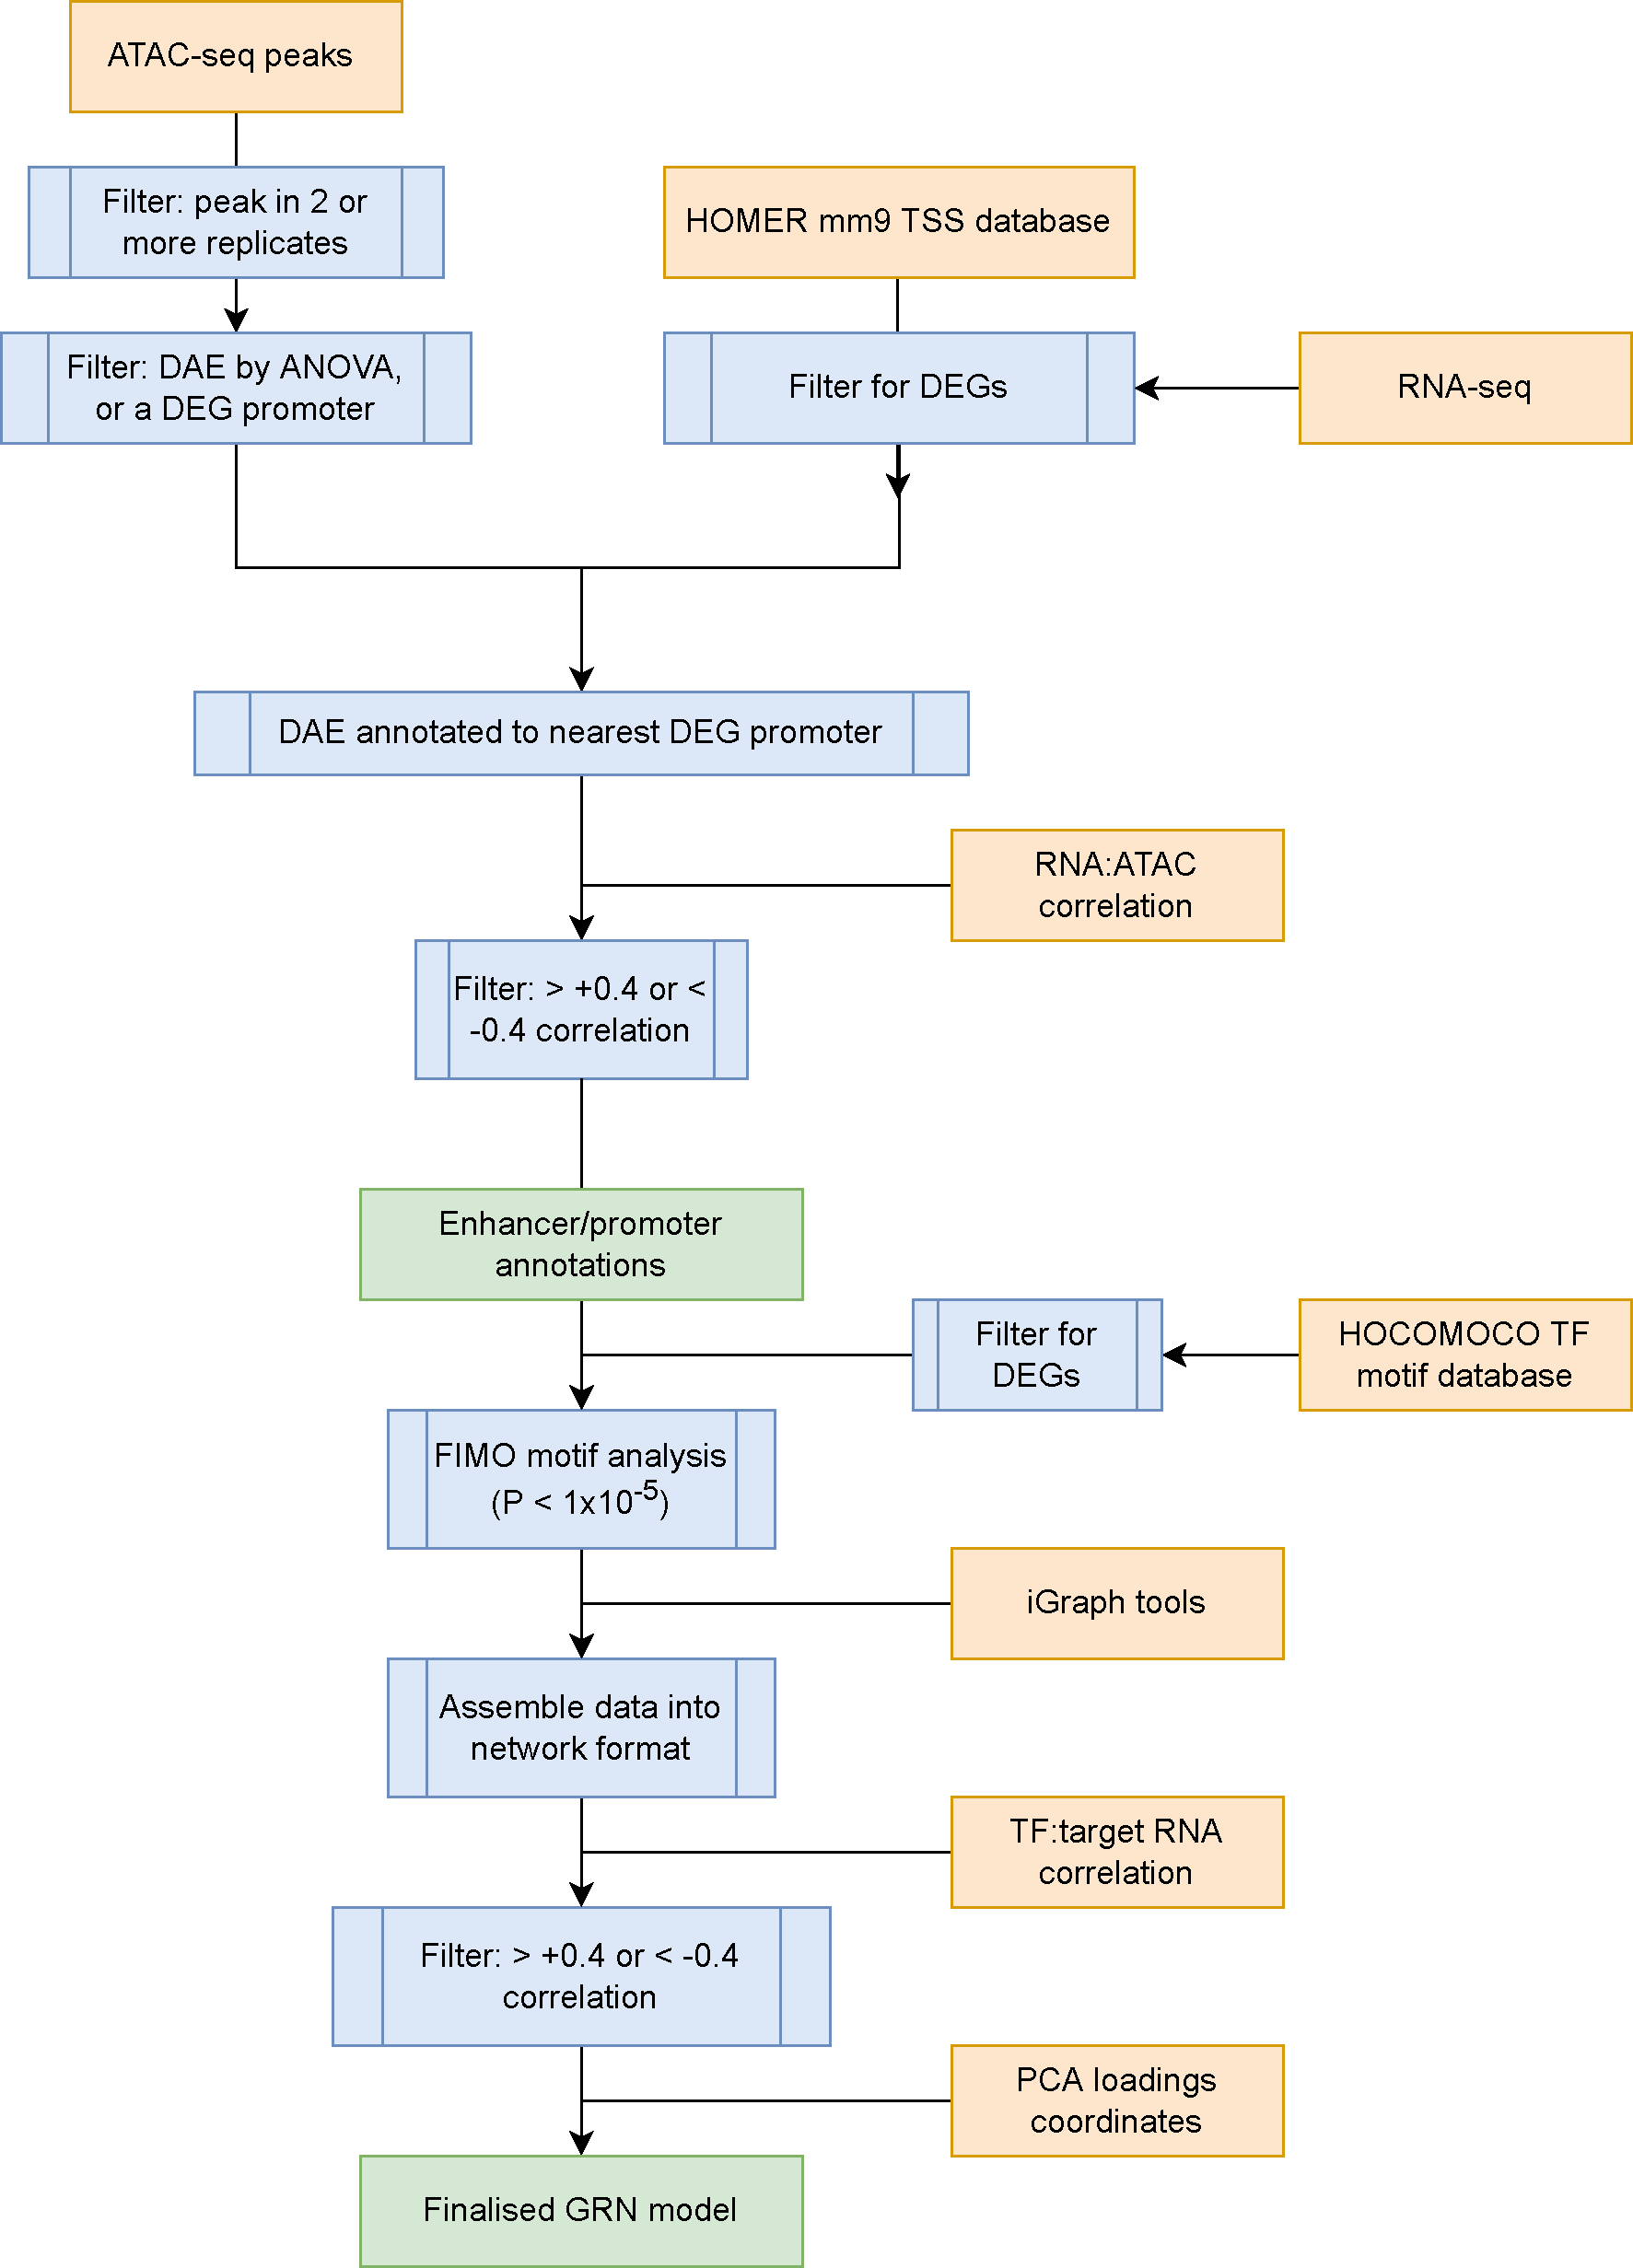
\includegraphics[width=0.8\textwidth,height=\textheight,keepaspectratio]{figures/appendix/app_eht-workflow.png}
    \caption[{Flow diagram explaining the integration of RNA-seq and ATAC-seq data to generate the EHT GRN model.}]
    {\textbf{Flow diagram explaining the integration of RNA-seq and ATAC-seq data to generate the EHT GRN model.} 
    Flow diagram schematic outlining the steps involved in the integration of RNA-seq and ATAC-seq data to generate the EHT GRN. Input data coloured orange; data processing steps coloured blue; data outputs coloured green.
    }
    \label{fig:app_eht-workflow}
\end{figure}
\clearpage

\begin{figure}[p]
    \centering
    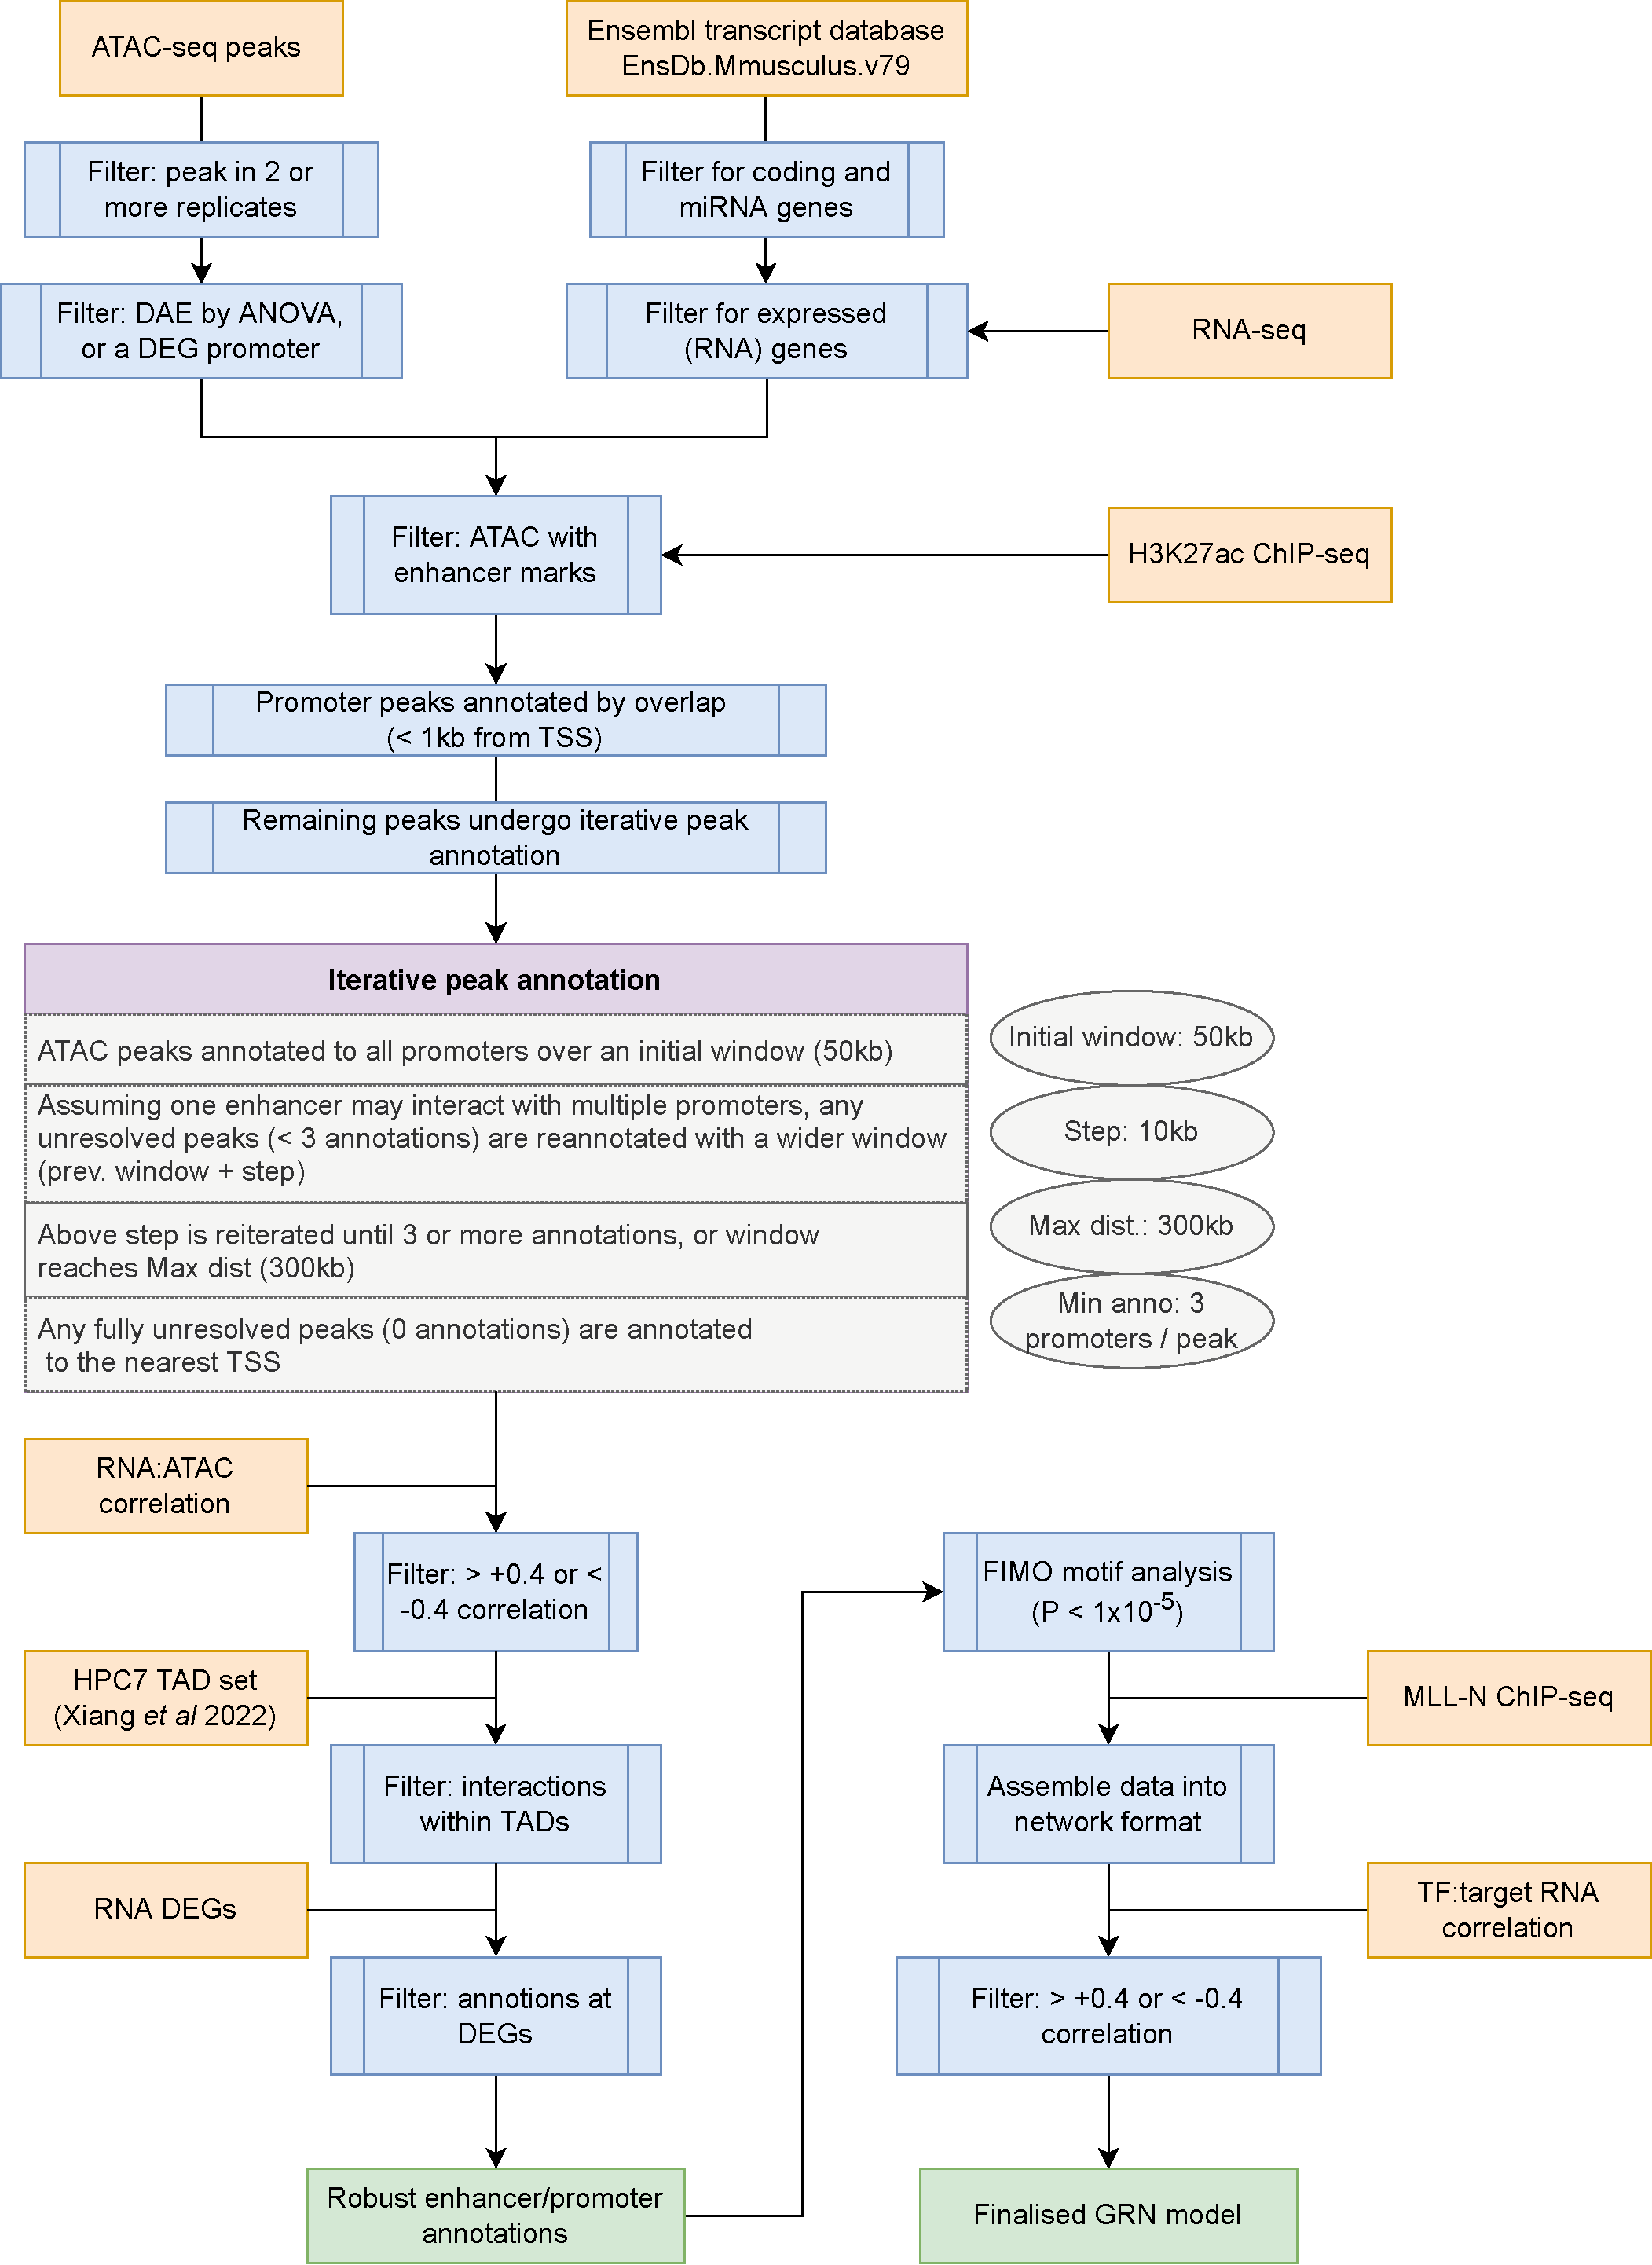
\includegraphics[width=0.8\textwidth,height=\textheight,keepaspectratio]{figures/appendix/app_methocult-workflow.png}
    \caption[{Flow diagram explaining the processing of ATAC-seq, RNA-seq and ChIP-mentation data to generate the MLL-AF9 GMP GRN.}]
    {\textbf{Flow diagram explaining the processing of ATAC-seq, RNA-seq and ChIP-mentation data to generate the MLL-AF9 GMP GRN.} 
    Flow diagram schematic outlining the steps involved in the processing and annotating of ATAC-seq data, and the integration of gene expression and ChIP-mentation data to generate the MLL-AF9 GMP GRN. Input data coloured orange; data processing steps coloured blue; data outputs coloured green.
    }
    \label{fig:app_methocult-workflow}
\end{figure}
\clearpage



%%%% Chapter 3 %%%%

\begin{figure}[p]
    \centering
    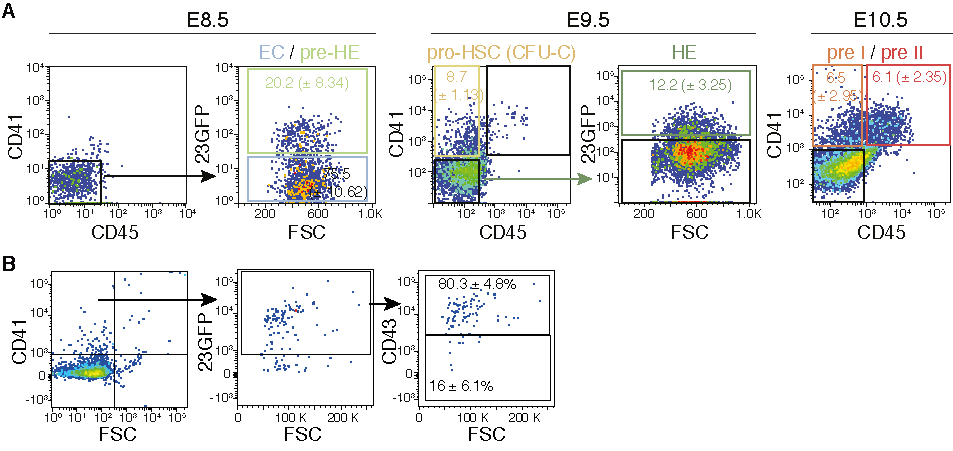
\includegraphics[width=\textwidth,height=\textheight,keepaspectratio]{figures/appendix/app_eht-sort-gates.png}
    \caption[{Flow cytometry panels for EHT haematopoietic population isolation.}]
    {\textbf{Flow cytometry panels for EHT haematopoietic population isolation.} 
    \textbf{(A)} Representative flow cytometry panels for the sorting of EHT populations for RNA-seq and ATAC-seq analysis. Flow cytometry panels are gated on Ter119\uneg{}VE-Cad\upos{} live cells.
    \textbf{(B)} Representative flow cytometry panels analysing E9.5 PAS from 23GFP embryos, showing the percentage of CD43\upos{} cells in the Ter119\uneg{}VE-Cad\upos{}CD41\upos{}CD45\uneg{} gate.
    \textit{Flow cytometry analyses performed by Gemma Swiers and Emanuele Azzoni (de Bruijn lab).}
    }
    \label{fig:app_eht-sort-gates}
\end{figure}
\clearpage


\begin{figure}[p]
    \centering
    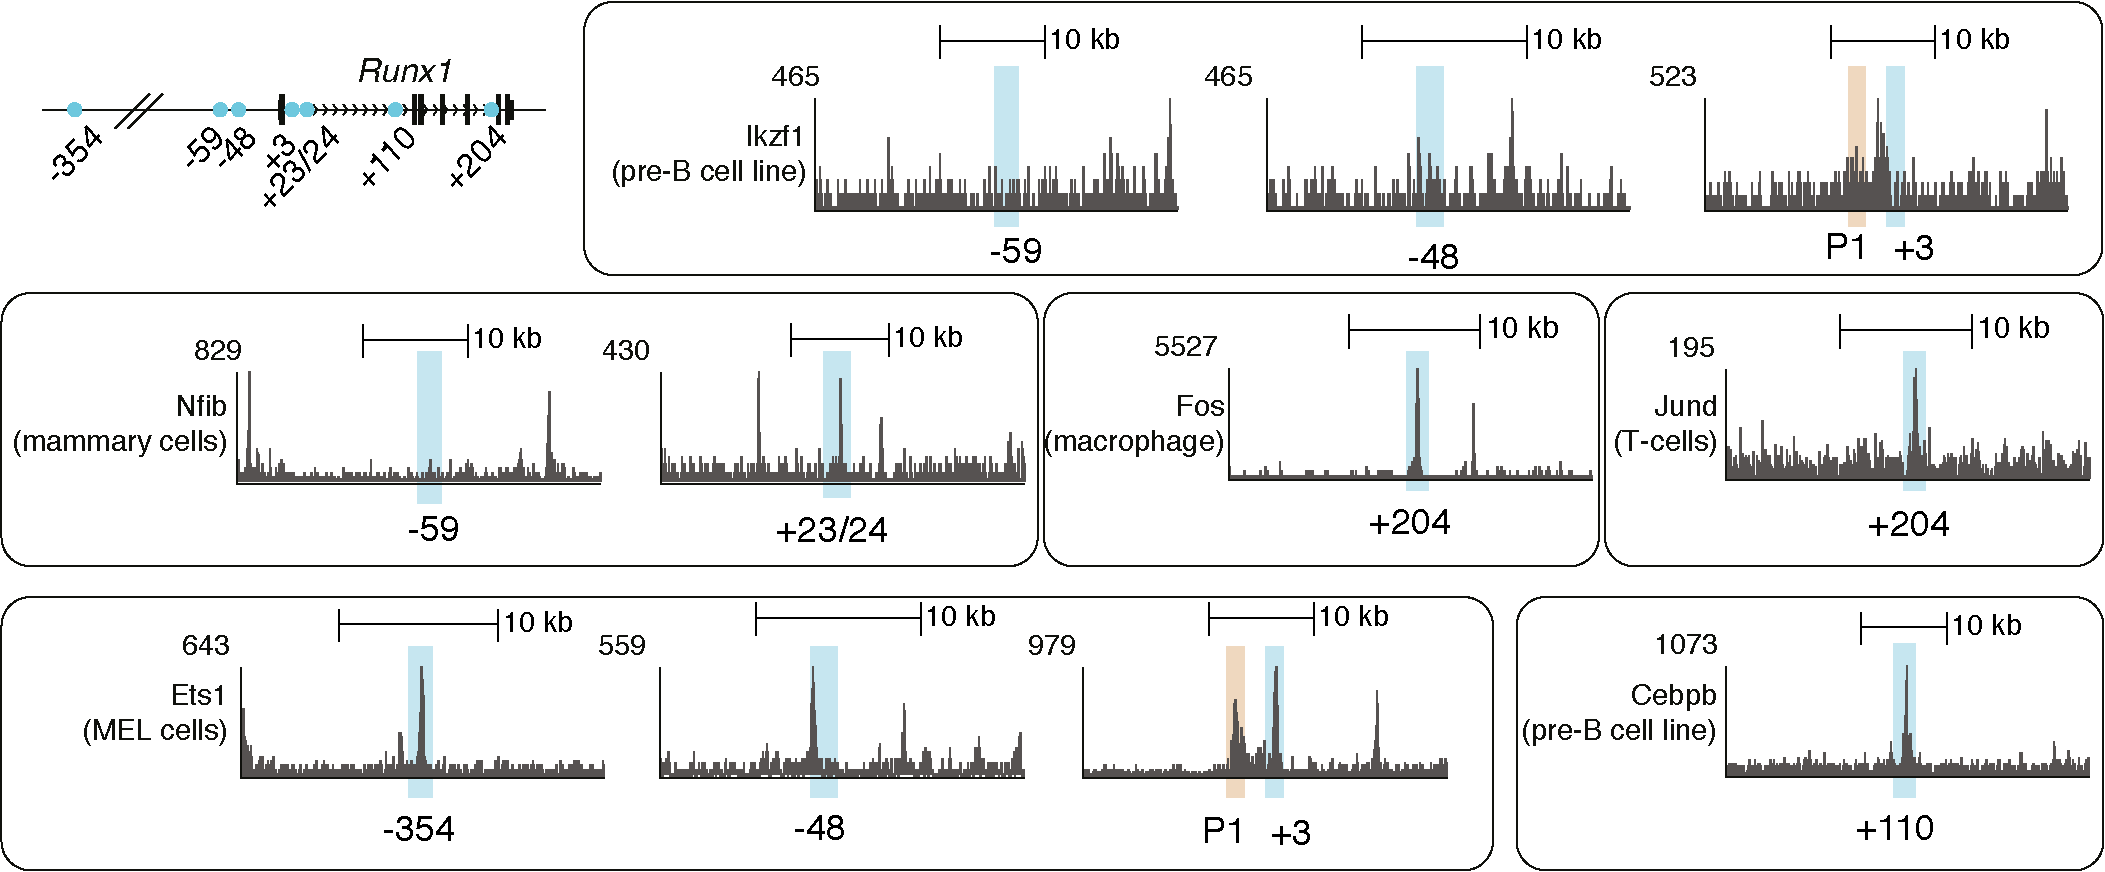
\includegraphics[width=\textwidth,height=\textheight,keepaspectratio]{figures/appendix/app_runx1-upstream-chip.png}
    \caption[{Published ChIP-seq validation of TF motifs.}]
    {\textbf{Published ChIP-seq validation of TF motifs.} 
    ChIP-seq tracks over \textit{Runx1} enhancers from reanalysed published ChIP-seq datasets. Schematic of \textit{Runx1} locus and relevant enhancers shown. Tracks are scaled to maximum signal of the window.
    }
    \label{fig:app_runx1-upstream-chip}
\end{figure}
\clearpage

%\begin{wrapfigure}{r}{0.5\textwidth}
%  \begin{center}
%    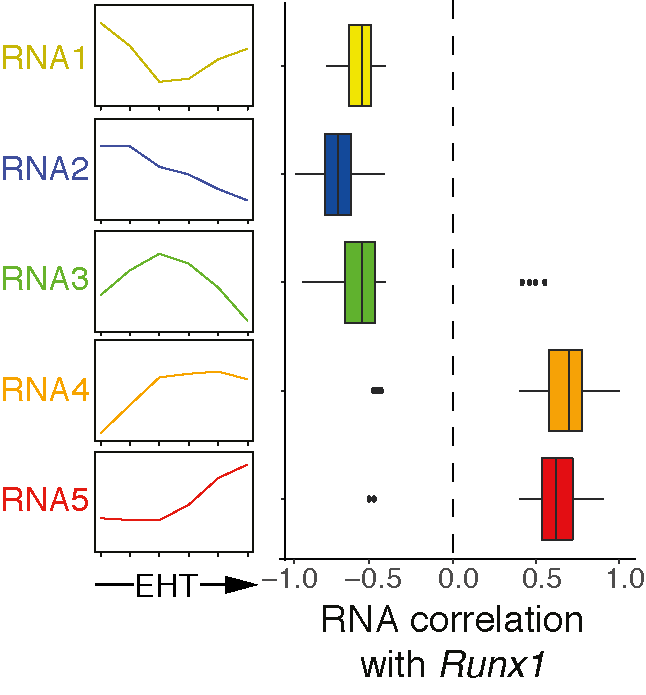
\includegraphics[width=0.48\textwidth]{figures/chapter3/ch3_runx1-cor.png}
%  \end{center}
%  \caption[{\textit{Runx1} correlation with expression modules.}]
%    {\textbf{\textit{Runx1} correlation with expression modules.} 
%    Boxplot summary of transcription correlation between \textit{Runx1} expression and Runx1 target genes, stratified by RNA-seq cluster (C1-5)
%    }
%    \label{fig:ch3_runx1-cor}
%\end{wrapfigure}

\begin{figure}[p]
    \centering
    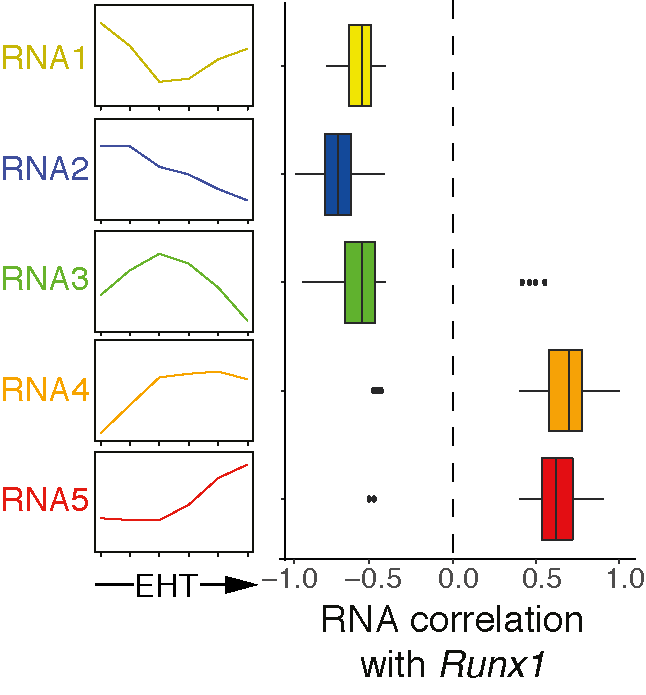
\includegraphics[width=0.7\textwidth,height=0.7\textheight,keepaspectratio]{figures/chapter3/ch3_runx1-cor.png}
    \caption[{\textit{Runx1} correlation with predicted Runx1 targets, across EHT GRN modules.}]
    {\textbf{\textit{Runx1} correlation with predicted Runx1 targets, across EHT GRN modules.} 
    Boxplot summary of transcription correlation between \textit{Runx1} expression and Runx1 target genes, stratified by RNA expression module (RNA1-5). 
    }
    \label{fig:app_runx1-cor}
\end{figure}
\clearpage

\begin{figure}[p]
    \centering
    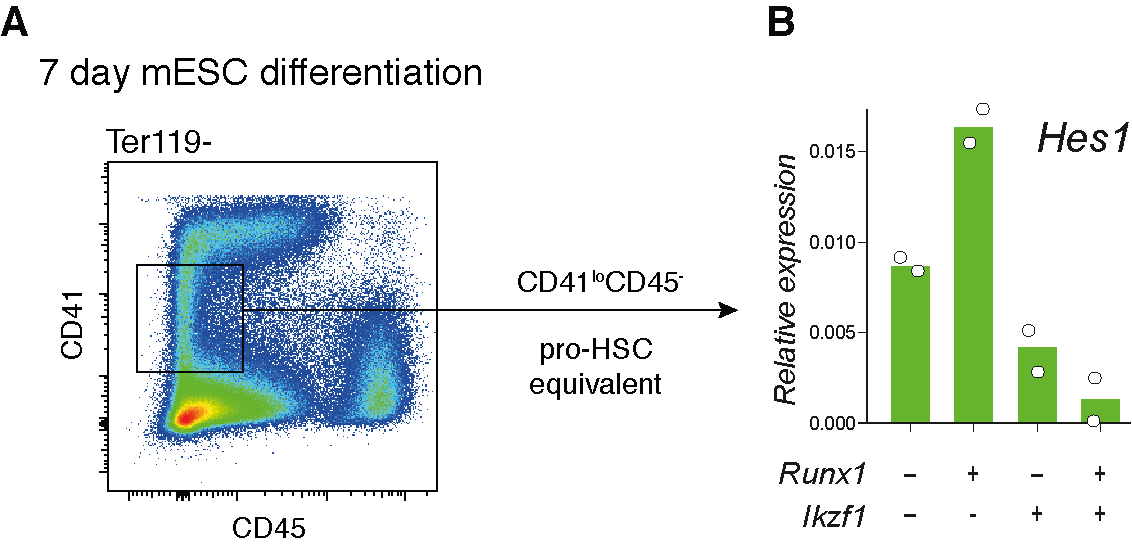
\includegraphics[width=\textwidth,height=\textheight,keepaspectratio]{figures/appendix/app_notch-ffl-validation.png}
    \caption[{Functional validation of the Runx1:Ikzf1:\textit{Hes1} FFL.}]
    {\textbf{Functional validation of the Runx1:Ikzf1:\textit{Hes1} FFL.} 
    \textbf{(A)} Representative flow cytometry panel for analysis at day 7 of haematopoietic differentiation of mESC lines. Analyses were performed on Ter119\uneg{} live cells.
    \textbf{(B)} qRT-PCR assaying Hes1 expression at day 7 of mESC differentiation in Runx1-ERt2::Ikzf1\textsuperscript{+/+} and Runx1-ERt2::Ikzf1\textsuperscript{-/-} mESC lines, with or without +4-OHT. Expression normalized to Atp5a1 and Gapdh. N = 2 differentiations. Conditions are represented on the x axis as Runx1 and Ikzf1 status, where + indicates active, and - indicates inactive. Labels include Runx1- (-4-OHT), Runx1+ (+4-OHT), Ikzf1- (Runx1-ERt2::Ikzf1\textsuperscript{-/-} cell line), and Ikzf1+ (Runx1-ERt2::Ikzf1\textsuperscript{+/+} cell line). 
    \textit{Data in this figure was generated by Lucas Greder (de Bruijn lab)}
    }
    \label{fig:app_notch-ffl-validation}
\end{figure}
\clearpage

 %We established a system in which we can perturb \textit{Runx1} and \textit{Ikzf1} activity during mESC haematopoietic differentiations. We fused an ERt2 domain to the C-terminus of endogenous \textit{Runx1} in mESCs (\textit{Runx1-ERt2}), to allow inducible control of Runx1 localisation from the cytoplasm (-4-OHT) to the nuclear (+4-OHT), which we confirmed by immunofluorescence imaging (Supplementary Figure S7A, B). We additionally took this cell line and induced a frameshift mutation in exon 3 of \textit{Ikzf1} (Supplementary Figure S7C), which is shared by all isoforms \citep{marke_many_2018} (\textit{Runx1-ERt2::Ikzf1\textsuperscript{-/-}}). As Ikzf1 is critically required for the B cell lineage, we looked for defects in the ability for these cell lines to generate B cells \citep{wang_disruption_1996, nichogiannopoulou_defects_1999}.

%%%% Chapter 4 %%%%

\begin{figure}[p]
    \centering
    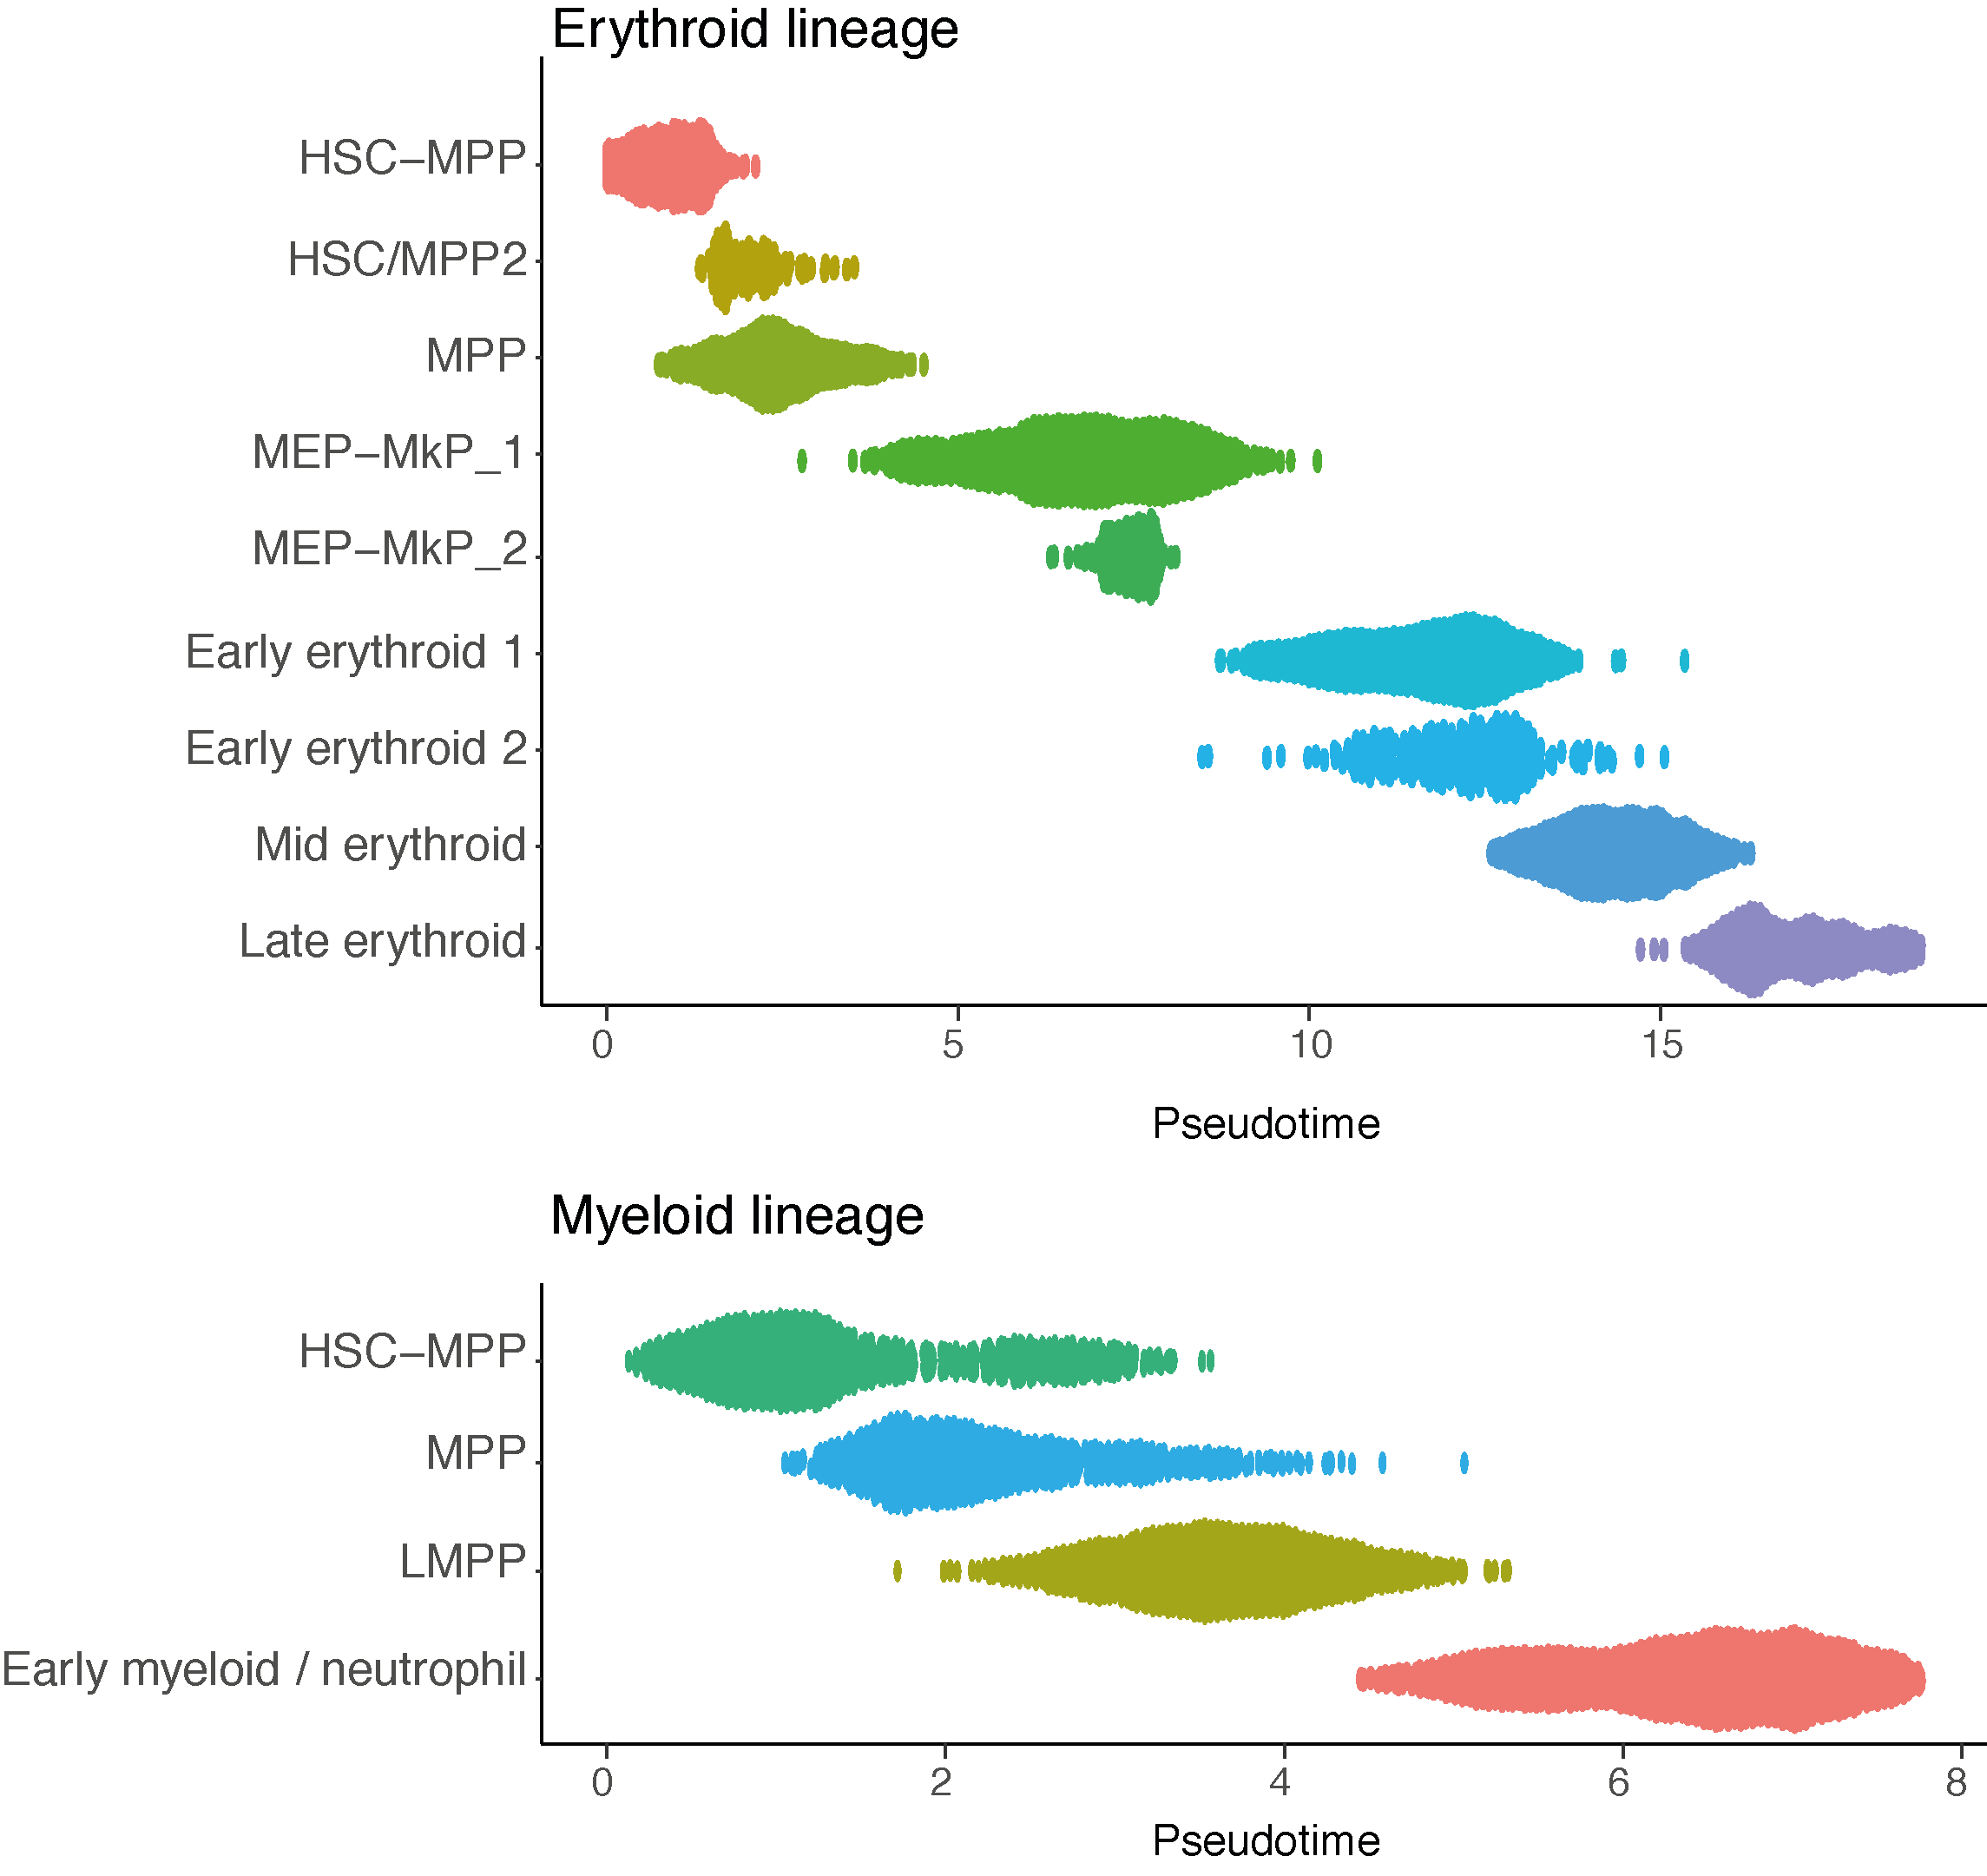
\includegraphics[width=\textwidth,height=\textheight,keepaspectratio]{figures/appendix/app_multiome-other-pseudo.png}
    \caption[{Sc-multiome erythroid and myeloid (neutrophil) lineages.}]
    {\textbf{Sc-multiome erythroid and myeloid (neutrophil) lineages.} 
    Erythropoiesis and Myelopoiesis assigned cells ordered by slingshot pseudotime, stratified by assigned cluster as in Figure \ref{fig:ch4_multiome-clusters}.
    }
    \label{fig:app_multiome-other-pseudo}
\end{figure}
\clearpage

\begin{figure}[p]
    \centering
    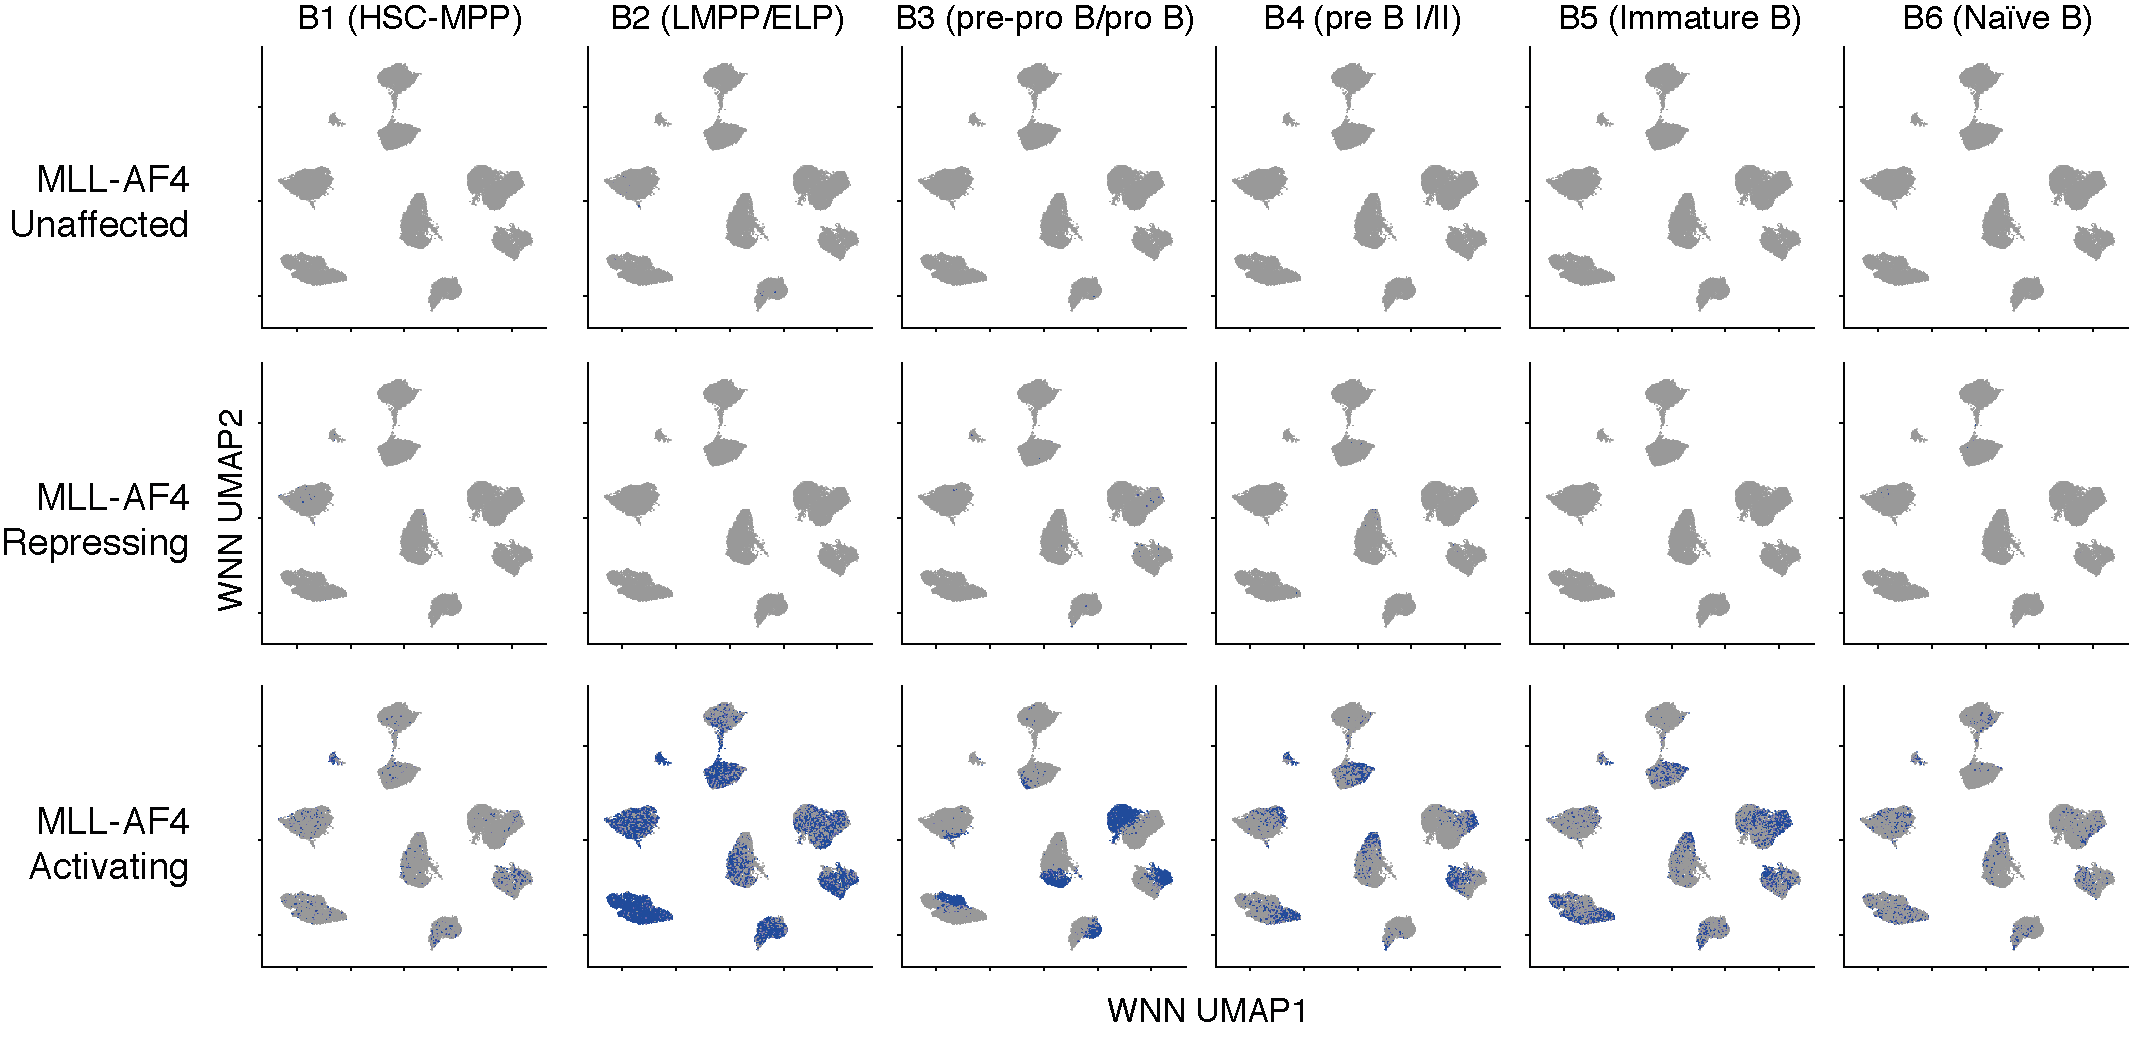
\includegraphics[width=\textwidth,height=\textheight,keepaspectratio]{figures/appendix/app_multiome-grn-enrich.png}
    \caption[{MLL-AF4 GRN enrichment in normal FBM and FL.}]
    {\textbf{MLL-AF4 GRN enrichment in normal FBM and FL.} 
    ALL blast UMAPs, annotated with cells passing AUCell thresholds marking enrichment for MLL-AF4 GRN regulated genes (MLL-AF4 activating or repressing) in each B lymphopoiesis signature as in Figure \ref{fig:ch4_multiome-tradeseq}.
    }
    \label{fig:app_multiome-grn-enrich}
\end{figure}
\clearpage


%%%% Chapter 5 %%%%

\begin{figure}[p]
    \centering
    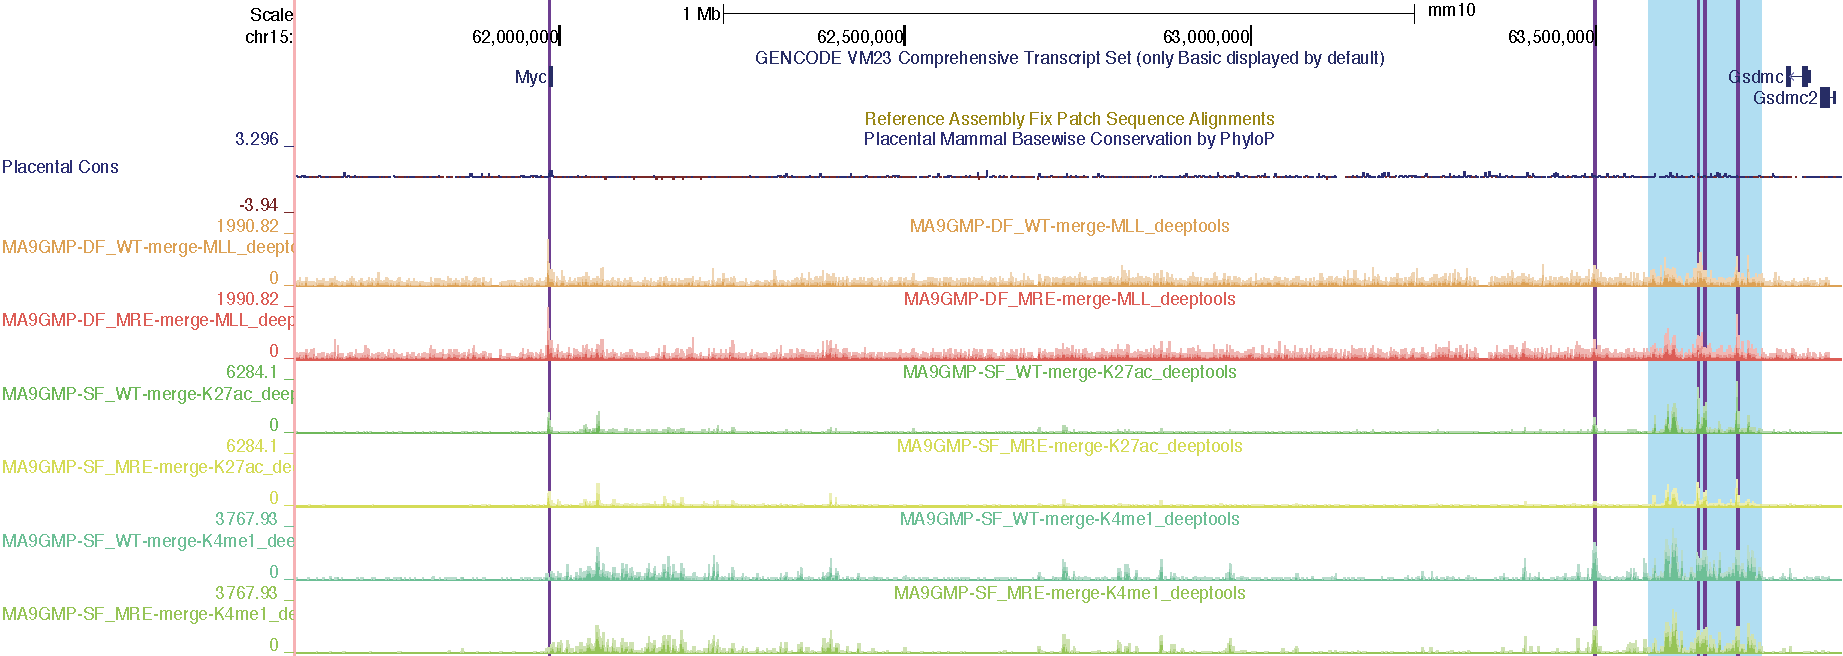
\includegraphics[width=\textwidth,height=\textheight,keepaspectratio]{figures/appendix/app_myc-annotation.png}
    \caption[{\textit{Myc} enhancer annotations in MLL-AF9 GMPs.}]
    {\textbf{\textit{Myc} enhancer annotations in MLL-AF9 GMPs.} 
    UCSC tracks showing MLL-N, H3K27ac, and H3K4me1 ChIP-mentation tracks. Replicates were merged for visualisation. Blue highlight indicates 1.7 mb superenhancer, and purple highlights indicate enhancers elements annotated to \textit{Myc}.
    }
    \label{fig:app_myc-annotation}
\end{figure}





%ELBOW
 %   \textbf{(C)} Plot to find optimal number of clusters for \textit{k}-means, showing relationship between remaining variation within clusters (total within-clusters sum of squares) and number of clusters (k). 
